	\documentclass[12pt,a4paper,titlepage,openany]{report}
\usepackage{zakljucna_FAMNIT_1_stopnja_MA_MEF_EN_2016}
\usepackage{enumitem}  
\DeclareMathOperator{\Cdim}{Cdim}

% Head of document:

\fancyhf{}
\lhead[]{{\fontsize{9.3}{12}\selectfont
Avdullahu A. Representations of Graphs as Induced Subgraphs of Hamming Graphs.\\
\noindent Univerza na Primorskem, Fakulteta za matematiko, naravoslovje in informacijske tehnologije, year}}
\chead[]{\fancyplain{}{}}
\rhead[]{\fancyplain{\thepage}
{\thepage}}
\cfoot[]{\fancyplain{}{}}
\lfoot[]{\fancyplain{}{}}
\rfoot[]{\fancyplain{}{}}
\normalsize

%%%%%%%%%%%%%%%%%%%%%%%%% BEGINNING OF DOCUMENT %%%%%%%%%%%%%%%%%%%%%%%%%%%%%%%%%%%%%%%%%%5

%%%%%%%%%%%%%%%%%%%%%%%%% Title page %%%%%%%%%%%%%%%%%%%%%%%%%


\begin{document}
\pagenumbering{Roman}
\pagestyle{empty}
\begin{center}
\noindent \large UNIVERZA NA PRIMORSKEM\\
\large FAKULTETA ZA MATEMATIKO, NARAVOSLOVJE IN\\
INFORMACIJSKE TEHNOLOGIJE


\normalsize
\vspace{5.5cm}
Seminar - uvod v raziskovalno delo\\
(Seminar - Introduction to Research Work)\\
\textbf{\large Predstative grafov kot induciram podgrafi Hammingorih grafov}\\
\normalsize
(Representations of Graphs as Induced Subgraphs of Hamming Graphs)\\
\end{center}

\begin{flushleft}
\vspace{5cm}
\noindent Ime in priimek: Arber Avdullahu
% add your first name and last name in the line above
\\
\noindent \v Studijski program: Matematika
% add your study program in the line above
\\
\noindent Mentor: prof. dr. Martin Milani\v c
% add the academic title, first name, and last name of your mentor in the line above
\\
\noindent Somentor: prof. dr. Marcelo Mydlarz
% if you have a co-mentor, add his/her academic title, first name, and last name in the line above
% if you do not have a co-mentor, delete the line above and the line below
\\
\end{flushleft}

\vspace{4cm}
\begin{center}
\large \textbf{Koper, April 2019}
% add the month and year of submission of your final project paper
\end{center}
\newpage

\pagestyle{fancy}
%%%%%%%%%%%%%%%%%%%%%%%%%%%%%%% Key words documentation (Slovene and English) %%%%%%%%%%%

\section*{Klju\v cna dokumentacijska informacija}

\medskip
\begin{center}
\fbox{\parbox{\linewidth}{
\vspace{0.2cm}
\noindent
Ime in PRIIMEK:\vspace{0.5cm}\\
Naslov seminarske naloge:\vspace{0.5cm}\\
Kraj:\vspace{0.5cm}\\
Leto:\vspace{0.5cm}\\
\v Stevilo listov: \hspace{2cm} \v Stevilo slik: \hspace{2.6cm} \v Stevilo tabel:\hspace{2cm}\vspace{0.5cm}\\
\v Stevilo prilog: \hspace{1.9cm} \v Stevilo strani prilog: \hspace{1cm} \v Stevilo referenc:\vspace{0.5cm}\\
Mentor:\vspace{0.5cm}\\
Somentor:\vspace{0.5cm}\\
Klju\v cne besede:\vspace{0.5cm}\\
Math.~Subj.~Class.~(2010):\vspace{0.5cm}\\
{\bf Izvle\v cek:}\\
Izvle\v cek predstavlja kratek, a jedrnat prikaz vsebine naloge. V najve\v c 250 besedah naka\v zemo problem, metode, rezultate, klju\v cne ugotovitve in njihov pomen.
\vspace{0.2cm}
}}
\end{center}

\newpage

\section*{Key words documentation}

\medskip

\begin{center}
\fbox{\parbox{\linewidth}{
\vspace{0.2cm}
\noindent
Name and SURNAME: Arb\"er Avdullahu\vspace{0.5cm}\\
Title of term project paper: Representations of Graphs as Induced Subgraphs of Hamming Graphs\vspace{0.5cm}\\
Place: Koper\vspace{0.5cm}\\
Year: 2019\vspace{0.5cm}\\
Number of pages:\hspace{1.6cm} Number of figures:\hspace{2.2cm} Number of tables:\vspace{0.5cm}\\
Number of appendices:\hspace{0.6cm} Number of appendix pages:\hspace{0.8cm}Number of references:\vspace{0.5cm}\\
Mentor:  Prof. Martin Milani\v c, PhD\vspace{0.5cm}\\

Co-Mentor: Prof. Marcelo Mydlarz, PhD\vspace{0.5cm}\\
Keywords: graph, Hamming graph, KP-labeling, gridline graph, induced embedding, Cartesian dimension, Hamming dimension\vspace{0.5cm}\\
Math.~Subj.~Class.~(2010): 05C15, 22D30, 97K30\vspace{0.5cm}\\
{\bf Abstract:} In this final project paper we consider induced subgraphs of Hamming graphs. The representation of graphs as induced subgraphs of a larger graph with a special structure often allows a better understanding of the properties of the given graphs. Using embeddings into Cartesian products of quotient graphs Klav\v zar and Peterin characterized induced subgraphs of Hamming graphs in 2005. We study the Cartesian dimension defined by Milani\v c, Mur\v si\v c and Mydlarz in 2007. The study consist of structural, algorithmic, and complexity aspects of the Cartesian dimension of graphs. We also take a quick look at Hamming dimension defined by Klav\v zar, Peterin and Zemlji\v c in 2013.
\vspace{0.2cm}
}}
\end{center}




%%%%%%%%%%%%%%%%%%%%%%%%%%%%%%% Acknowledgement %%%%%%%%%%%%%%%%%%%%%%%%%%%%%%%%%%%%%

\newpage
\section*{Acknowledgement}

Here we thank all involved with our term project paper, that is, persons or institutions that helped us in our work and/or made it possible.
We can also thank the mentor and the co-mentor (if there is one)

%%%%%%%%%%%%%%%%%%%%%%%%%%%%% Table of contents, list of figures, etc. %%%%%%%%%%%%%%%%%%%%%%%%%%%%%%
\newpage

\tableofcontents
\addtocontents{toc}{\protect\thispagestyle{fancy}}
% if there are no tables in your final project paper, delete the following three lines
\newpage
\listoftables
\addtocontents{lot}{\protect\thispagestyle{fancy}}
% if there are no figures in your final project paper, delete the following three lines
\newpage
\listoffigures
\addtocontents{lof}{\protect\thispagestyle{fancy}}
\newpage
% Since the appendices are not numbered, we also do not want to show the dots to their (non-existing) page numbers.
\renewcommand{\cftdot}{}
\listofappendices
\thispagestyle{fancy}
\newpage

\chapter*{List of Abbreviations}
\thispagestyle{fancyplain}
\begin{longtable}{@{}p{1cm}@{}p{\dimexpr\textwidth-1cm\relax}@{}}
\nomenclature{{\it i.e.}}{that is}
\nomenclature{{\it e.g.}}{for example}
\end{longtable}
\newpage

\normalsize

%%%%%%%%%%%%%%%%%%%%%%%%%%%%%%%%%% Chapters: %%%%%%%%%%%%%%%%%%%%%%%%%%%%%%%%%%%%%

% Hint: You might find it convenient to keep the contents of separate chapters in separate files, each in their own
% .tex file. They all have to be stored in the same folder as the main file. Each chapter is included with the \include command.
% Example: we can insert FirstChapter.tex and SecondChapter.tex as follows:
% \include{FirstChapter}
% \include{SecondChapter}
\chapter{Introduction}
\thispagestyle{fancy}
\pagenumbering{arabic}

Representating graphs as induced subgraphs of a larger graph with a special structure often leads to a better understanding of the properties of a given graph. 

In this paper, we will take a closer look at Hamming graphs. Hamming graphs are named after the mathematician Richard Hamming and they are used in various branches of mathematics and computer science. By definition, they are the Cartesian products of complete graphs. In order to solve the problem of efficiently recognizing whether a graph is a Hamming graph, we can use the prime factorization algorithms with respect to the Cartesian product. Imrich and Klav\v zar present an algorithm for recognizing Hamming graphs which is linear in both time and space $\sim$\cite{Imrich}.\newline
Hamming graphs have been characterized in various way. Mulder in \cite{Mulder} has characterized the Hamming graphs as interval-regular graphs with some additional properties. This is analogous to his characterization of hypercubes as bipartite interval-regular graphs \cite{Mulder}.

 In \cite{Egawa}, Egawa showed that if $G$ is a connected graph with the same proper convex subgraphs as a Hamming graph where all $r$ complete graphs have the same size $n$, then $|V(G)|\geq n^r$ with equality if and only if $G$ is isomorphic to Hamming graph. 
 
 In \cite{Mollard}, Mollard gives two characterization of Hamming graphs, the first one is the analogous of the charazterization of the hypercube as $(0,2)$-graph (a connected graph in which any two vertices have 2 common neighbours or none at all) of maximal order; the second introduces the notion of quasi-interval. Isometric subgraphs of Hamming graphs, which are called partial Hamming graphs, have also been extensively studied by now. \newline
Graham and Winkler \cite{Graham} proved that every graph has a representation as an isometric subgraph of a Cartesian product graph. The key construction is based on embedding into Cartesian products of the so-called quotient graphs with respect to a certain relation defined on the edge set of a graph. Feder \cite{Feder} followed with a similar approach in order to obtain such representations for stronger embeddability conditions: 2-isometric representation, weak retract representation, and Cartesian prime factorization. 

A different direction was taken by Klav\v zar and Peterin in \cite{Iztok}, treating isometry as the strongest property, and considering subgraphs, induced subgraphs, and isometric subgraphs of Hamming graphs. They showed, roughly speaking, that embeddings into Cartesian product of quotient graphs can be applied also to subgraphs and induced subgraphs of Hamming graphs. \newline
Several graph "dimensions"(or: invariants) based on embeddings into product graphs have been studied by now. In the work done by Milani\v c, Mur\v si\v c, and Mydlarz in \cite{Milanic}, they studied the question about how difficult is it to determine if a given graph $G$ can be realized in $\mathbb{R}^d$ so that vertices are mapped to distinct points and two vertices are adjacent if and only if the corresponding points are on a common line that is parallel to some axis.
Any such mapping is referred as a $d$-realization of $G$ and we say that a graph is $d$-realizable if it has a $d$-realization. A graph $G$ is $d$-realizable if and only if it is an induced subgraph of a Cartesian product of complete graphs and the minimum non-negative integer $d$ such that $G$ is $d$-realizable is defined as Cartesian dimension of G defined in \cite{Milanic}, $d$-realizable graphs were studied under different names such as arrow graphs in \cite{Cook}, $(d - 1)$-plane graphs and $(d -1)$-line graphs of $d$-partite $d$-uniform hypergraphs in \cite{Bermond}, $d$-dimensional cellular graphs in \cite{Gurvich}, $d$-dimensional chess board graphs in \cite{Staton}, and $d$-dimensional gridline graphs in \cite{Peterson}.\newline

Recently, Sangha and Zito studied $d$-realizable graphs in the more general context of the so-called Line-of-Sight (LoS) networks in \cite{Zito}. Line of Sight (LoS) networks offer a model of wireless communication that incorporates visibility constraints. Vertices of such networks can be embedded in finite $d$-dimensional grids of size $n$, and two vertices are adjacent if they share a line of sight and are at a distance of less than $\omega$, where two points $x=(x_1, \ldots,x_d)$ and $x'=(x_1',\ldots ,x_d')$ share a line of sight if there exists some $j\in \{1,\ldots,d\}$ such that $x_i=x_i'$ for all $i\in \{1,\ldots,d\} \symbol{92} \{j\}$. They studied large independent sets in LoS networks. They proved that the computational problem of finding a largest independent set can be solved in polynomial time for one dimensional LoS networks. However, for $d \geq 2$, the (decision version of) the problem becomes NP-hard for any fixed $\omega \geq 3$ and even if $\omega$ is chosen to be a function of $n$ that is $O(n^{1-\epsilon})$ for any fixed $\epsilon>0$. In addition they showed that the problem is also NP-hard when $\omega = n$ for $d \geq 3$. This result extends earlier work which demonstrated that the problem is solvable in polynomial time for gridline graphs when $d = 2$. For the small-dimensional cases, $d \in \{2, 3\}$, Peterson suggested an application of $d$-realizable graphs to robotics in \cite{Peterson}: if the movement of a robot is restricted to be along axis-parallel directions only and turns are allowable only at certain points, then a shortest path in a $d$-realized graph gives the number of turns required.\newline
The dimension of a Hamming graph is the number of its factors, that is, the number of coordinates of its vertices.\newline
Another graph dimension defined in \cite{Sandi}, the Hamming dimension of a graph $G$ is introduced as the largest dimension of a Hamming graph into which $G$ embeds as an irredundant induced subgraph, which came as the need in order to significantly increase the number of graphs with a non-trivial dimension that comes from the Cartesian product of graphs as most of graph dimensions do not attain large values.
\newline
In this project paper we will take a closer look at representations of graphs as induced subgraphs of Hamming graphs. In Chapter \ref{kp-chapter} we will present the work done by Klav\v zar and Peterin, including a characterization of induced subgraphs of Hamming graphs. The main result in that section is a necessary and sufficient condition for a graph to be an induced subgraph of a ($d$-dimensional) Hamming graph.\newline In Chapter \ref{cdim-chapter} we discuss the properties of Cartesian dimension, an invariant introduced defined by Milani\v c, Mur\v si\v c, and Mydlarz. We will see the properties of Cartesian dimension and how it is related with what was done in Chapter \ref{kp-chapter}. Graphs having dimension 0,1 or 2 are well understood, while determining whether a graph has Cartesian dimension at most 3 is NP-complete. We also analyze Cartesian dimension of some special graphs.\newline
In Chapter \ref{hdim-chapter} we shortly introduce the definition of Hamming dimension, following \cite{Sandi}. We will present some bounds for the Hamming dimension of Sierpi\'nski graphs without proofs.



\chapter{Preliminaries}
\thispagestyle{fancy}

Before we start with the results, we will fix the terminology used in the project paper and summarize some basic result about graphs. We only consider finite, undirected, and simple graphs without isolated vertices.

 A graph consist of vertices which are connected by edges, and we write a graph $G$ as $G=(V,E)$, where $V$ is the vertex set and $E$ is the edge set in $G$. If $G=(V,E)$, we write $V(G)=V$ and $E(G)=E$. We define $G-S$ for $S\subseteq V(G)$, as $V(G)\backslash S$ and $G-F$ for $F\subseteq E(G)$, as $E(G)\backslash F$. The degree of a vertex is the number of edges that are incident to the vertex, the distance between two vertices $u$ and $v$ in a graph $G$ is the number of edges in a shortest path connecting them and we denote it by $d_G(u,v)$. The neighborhood of a vertex $v$ in a graph $G$ is the subgraph of $G$ induced by all vertices adjacent to $v$
A neighbourhood in which vertex $v$ itself is included is called the closed neighborhood. A cut-edge is an edge that when removed from a graph increases the number of components.

 Let us now go through some special family of graphs. A path $P_n$ is a graph whose vertices can be listed in the order $v_1, v_2,\ldots, v_n$ such that the edges are $\{v_i, v_{i+1}\}$ where $i = 1, 2,\ldots , n − 1$. A cycle $C_n$ in a graph is a non-empty trail in which the only repeated vertices are the first and last vertices, a cycle which has 3 edges is called triangle. A tree is a connected acyclic graph. A graph is bipartite if the vertices can be partitioned into two sets $V_1$ and $V_2$ such that all edges go only from $V_1$ to $V_2$(no edges go from $V_1$ to $V_1$ or from $V_2$ to $V_2$). A complete graph is a graph with $n$ vertices and an edge between every two vertices, it is denoted by $K_n$. A induced subgraph of $G$ is graph consisting of a subset of the vertices of a graph $G$ together with any edges whose endpoints are both in this subset. Figure \ref{diaclaw} shows the diamond which is a $K_4$ minus one edge and the claw graphs which is $K_{1,3}$.

\begin{figure}[h]
\begin{center}
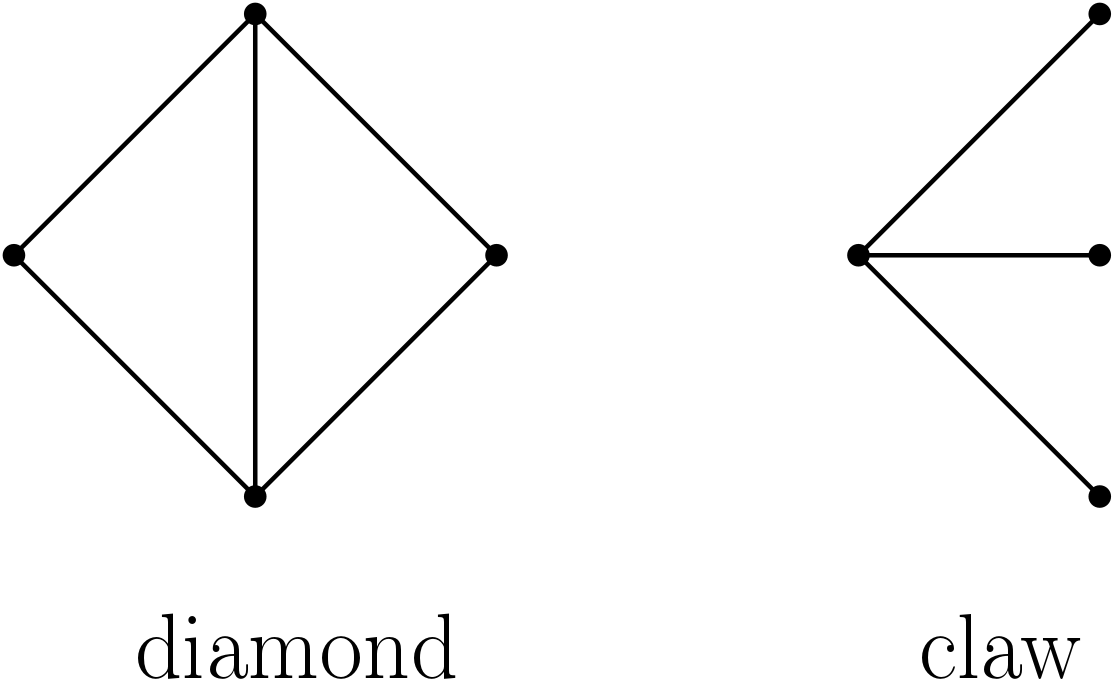
\includegraphics[width=0.5\linewidth]{figures/diaclaw.png}
\end{center}
\caption{The diamond and the claw.}\label{diaclaw}
\end{figure}

Let $\mathcal{F}$ A graph $G$ is said to be $\mathcal{F}$-free if no induced subgraph of $G$ is isomorphic to a graph from $\mathcal{F}$. A clique in a graph is a set of pairwise adjacent vertices, a maximal clique is a clique that it is not a subset of a larger clique. For a graph $G$, $L(G)$ denotes the line graph of $G$, the vertices of $L(G)$ are the edges of $G$ and two vertices of $L(G)$ are adjacent if the corresponding edges of $G$ are adjacent, see Figure \ref{linegraph} for an example. The adjacency matrix $A(G)=(a_{ij})_{i,j}^n$ of a graph G with vertex set $\{ v_1,v_2,\ldots, v_n\}$ is a square symmetric (0,1)-matrix whose rows and columns correspond to the vertices of $G$ and $a_{ij} = 1$ if and only if vertices $v_i$ and $v_j$ are adjacent. The clique graph $K(G)$ of a graph $G$ has as its vertex set the maximal cliques of $G$, with two vertices adjacent whenever they have some vertex of $G$ in common.\newline
Given a graph $G$, a $d$-edge-labeling of $G$ is a mapping from $E(G)$ to some set $L$ of labels, where $|L| = d$. Given a $d$-edge-labeling of $G$ and a set $F \subseteq E(G)$,
we say that $F$ is monochromatic if the labeling is the same for any edge in $F$. An edge coloring of a graph $G$ is a mapping from $E(G)$ to some set $L$ of labels such that no two incident edges have the same label. In this case, labels may also be referred to as colors.  Unless stated otherwise, a labeling (or more precisely a $k$-labeling) of $G$ will always mean an edge-labeling (with $k$ labels).

\begin{figure}[h]
\begin{center}
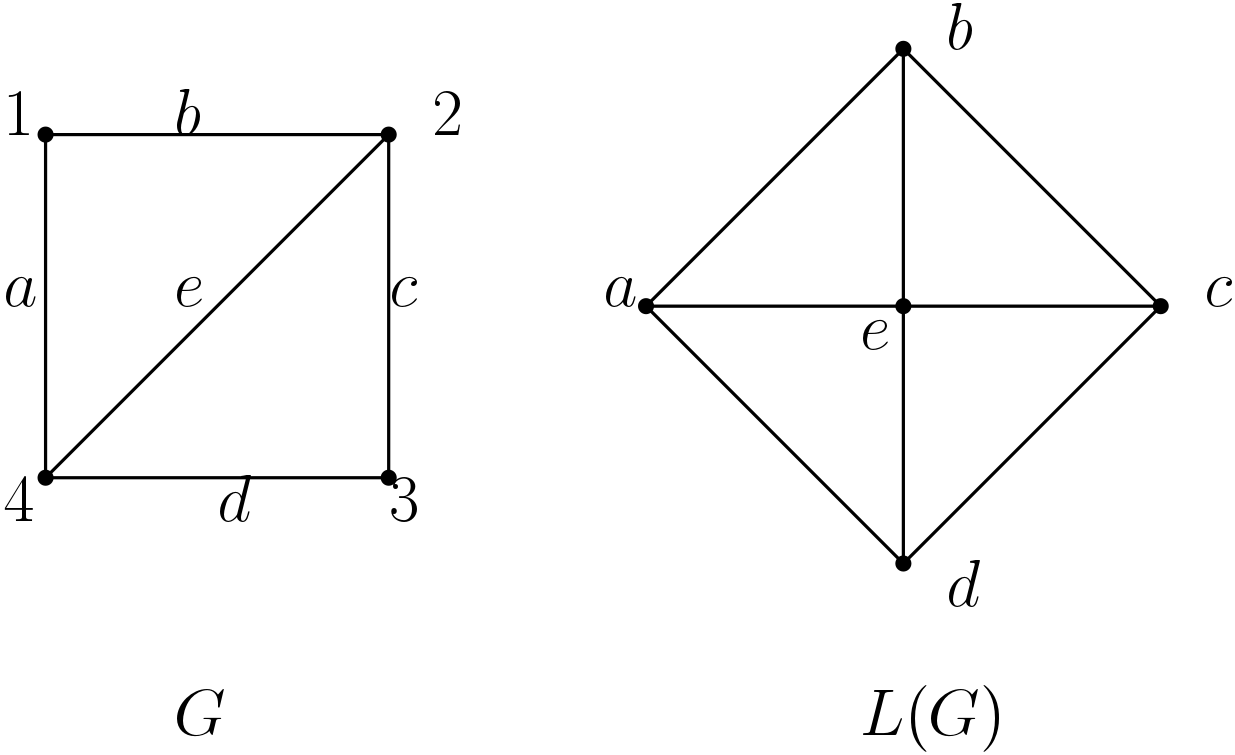
\includegraphics[width=0.7\linewidth]{figures/linegraph.png}
\end{center}
\caption{Line graph.}\label{linegraph}
\end{figure}
\medskip
We say that a graph $G$ is an irredundant subgraph of
$G_1\square G_2\square \ldots \square G_k$ if each $G_i$ has at least two vertices and any vertex of $G_i$ appears as a coordinate of some vertex of $G$. A subgraph $H$ of a graph $G$ is an isometric subgraph of $G$ if $d_H(u, v)=d_G(u, v)$ for each pair of vertices $u , v$ of $H$. 
\medskip








A \textit{decision problem} is a problem in which the set of instances divides into two sets depending on whether the answer is YES or NO.
In computational complexity theory, the following three classes of decision problems are of interest:
\begin{itemize}
\item {\it P} -- the set of decision problems that can be solved by a polynomial-time algorithm. Intuitively: $P$ is the set of problems that can be solved efficiently.
\item {\it NP} -- the set of decision problems with the following property:
If the answer is YES, then there exists a certificate that
enables us to verify this fact in polynomial time. Intuitively: NP is the set of problems for which we can
quickly verify a positive answer if we are given a solution.
\item {\it co-NP} -- the set of decision problems with the following property:
If the answer is NO, then there exists a certificate that
enables us to verify this fact in polynomial time.
\end{itemize}
The following lemma describes when an edge is cut-edge.
\begin{lemma}\label{cutedgecycle}
An edge of a graph G is a cut-edge if and only if it does not belong to any cycle.
\end{lemma}
\begin{proof} Take any edge $e = \{u, v\}$. We may assume with out loss of generality that $G$ is connected, since otherwise we can replace $G$ with the connected component of $G$ containg $e$. This will not affect any of the two properties of $e$ consider in the statement of the lemma.  Remove this edge from our graph. If the resulting graph has the same number of component as G, then there is some path from $u$ to $v$ not involving $e$;
consequently, if we add $e$ to the end of this path, we get a cycle. Thus, if $e$ is not a cut-edge, then $e$ belongs to a cycle.\newline
Conversely, suppose that $e = \{u, v\}$ lies in a cycle $C$. Then $P=C-e$ is a path from $u$ to $v$ that does not use $e$. Pick any two vertices $x, y$ in $G$; because $G$ is connected, there is a path from $x$ to $y$ in $G$. Take this path, and edit it as follows:
whenever the edge $e$ shows up, replace this with the path $P$ (or $P$ traced backwards, if needed). This then creates a walk from $x$ to $y$; by deleting cycles if necessary, this walk can be turned into a path from $x$ to $y$, and thus the graph $G-e$ is connected. So if $e$ is contained in a cycle, it is not a cut-edge.
\end{proof}
\chapter{Characterizing Subgraphs of Hamming Graphs}\label{kp-chapter}
\thispagestyle{fancy}

In this chapter we will talk about necessary and sufficent conditions for a graph to be an induced subgraph of a Hamming graph and some results regarding those conditions.  

\section{The definition of a KP-labeling}\label{kp-labeling-section}

Before presenting to the result we need to go through some definitions.
\newline

The Cartesian product $G\square H$ of graphs $G$ and $H$ is the graph with vertex set $V(G)\times V(H)$ in which a vertex $(a,x)$ is adjacent to a vertex $(b,y)$ whenever
$ab\in E(G)$ and $x=y$, or $a=b$ and $xy\in E(H)$. For a fixed vertex $a$ of $G$, the vertices $\{(a,x)|x\in V(H)\}$ induce a subgraph of $G \square H$ isomorphic to $H$, called an \textit{$H$-layer} of $G \square H$. Analogously we define \textit{$G$-layers}.\newline
More generally, the Cartesian product $G_1\square G_2 \square \ldots \square G_n$ of graphs $G_1,G_2,\ldots, G_n$ is the the graph with vertex set $V(G_1)\times V(G_2)\times \ldots \times V(G_n)$ in which a vertex $(u_1,u_2,\ldots, u_n)$ is adjacent to a vertex $(v_1,v_2,\ldots,v_n)$ whenever $u_iv_i\in E(G_i)$ and $u_j=v_j$ for every $j\in \{1,2,\ldots,n\}\backslash \{i\}$.\newline
The map $p_G:V(G\square H) \to G$ defined by $p_G(a,x)=a$, is called a projection. The image of an edge $(a,x)(b,y)$ under projection $p_G$ is an edge when $x=y$, and a vertex when $a=b$.\newline
Similarly we extended the definion, the projection of $p_G:V(G\square H_1\square H_2\square \ldots \square H_n) \to G$ is defined by $p_G(a,h_1,h_2,\ldots,h_n)=a$
\begin{figure}[h]\label{fig:cartProduct}
\begin{center}
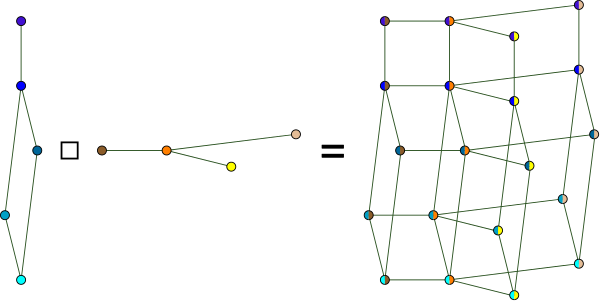
\includegraphics[width=0.75\linewidth]{figures/Graph-Cartesian-product.png}
\caption{The Cartesian product of graphs.}
\end{center}
\end{figure}
Cartesian products of complete graphs are known as Hamming graphs. But they can also be described as follows. For
$i=1,2,\ldots, n$ let $r_i\geq 2$ be given integers. Let $G$ be the graph whose vertices are the $n$-tuples $b_1b_2\cdots b_n$ with $b_i\in \{0,1,\ldots, r_i-1\}$. Two vertices are adjacent if the corresponding tuples differ in precisely one coordinate. The vertex set of $G$ is the same as that of $K_{r_1}\square K_{r_2}\square \ldots \square K_{r_n}$ and edges in $K_{r_1}\square K_{r_2}\square \ldots \square K_{r_n}$ between two vertices are exactly those that have same vertex in every graph $K_{r_i}$ but one. Since in complete graphs we have all possible edges, it is easy to see that $G$ and $K_{r_1}\square K_{r_2}\square \ldots \square K_{r_n}$ are isomorphic. For an edge $uv$ of
$H=K_{r_1}\square K_{r_2}\square \ldots \square K_{r_n}$ we define the color map $c:E(H)\rightarrow \{1,2,\ldots, n\}$ with $c(uv)=i$, where $u$ and $v$ differ in coordinate $i$.
\newline
Let $G$ be a connected graph and let $\mathcal{F}=\{F_1,F_2,\ldots, F_k\}$ be a partition of $E(G)$. The \textit{quotient graph} $G/ F_i$ has connected components of $G- F_i$ as vertices, two components $C$ and $C'$ being adjacent whenever there exists an edge of $F_i$ connecting a vertex of $C$ with a vertex of $C'$. For each $i$, define a map $f_i:V(G)\rightarrow V(G/ F_i)$ by $f_i(v)=C$, where $C$ is the component of $G- F_i$ containing $v$. Then let
$$f:V(G)\to V((G/ F_1)\square (G/ F_2)\square \ldots \square (G/ F_k))$$
be the natural coordinate-wise mapping, that is,
$$f(v)=(f_1(v),f_2(v),\ldots , f_k(v)).$$
We call $f$ the \textit{quotient map} of $G$ with respect to $\mathcal{F}$. Note that $f$ need not be one-to-one in general and that it is possible that some quotient graphs are the one vertex graph, an example is shown in Figure \ref{fnotonetoone}.
\begin{figure}[h]
\begin{center}
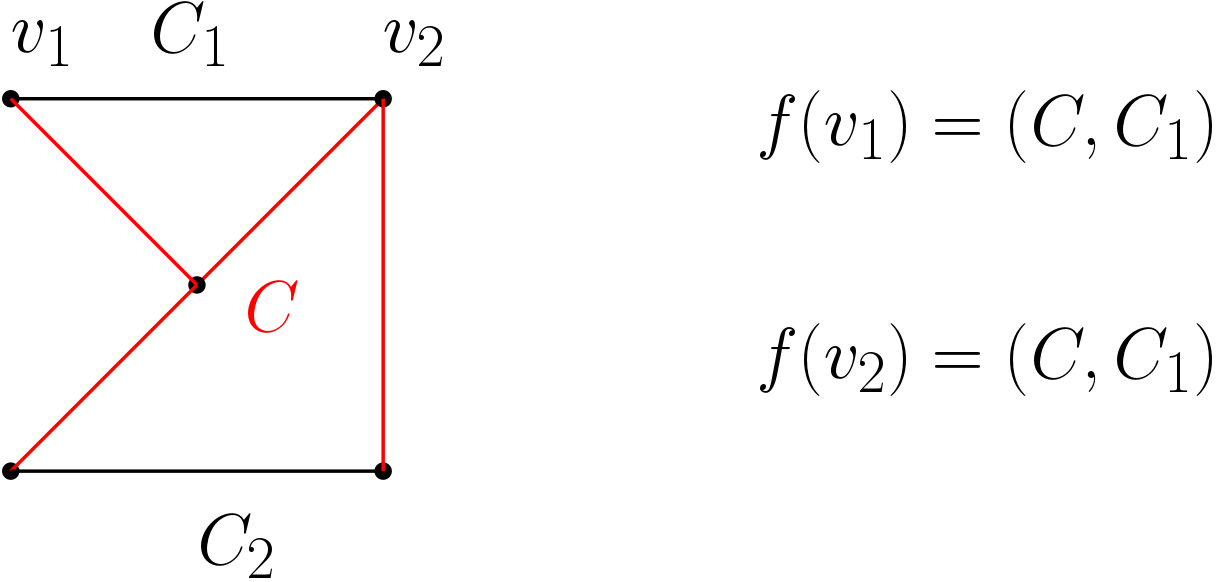
\includegraphics[width=0.75\linewidth]{figures/fnotonetoone.png}
\end{center}
\caption{An example of a graph such that the quotient map is not one-to-one}\label{fnotonetoone}
\end{figure}
 However, all the partitions $\mathcal{F}$ introduced later will lead to one-to-one mappings with non-trivial quotient graphs.\newline
A partition $\{F_1,F_2,\ldots ,F_k\}$ of $E(G)$ naturally leads to an edge-labeling $\ell:E(G)\to \{1,2,\ldots,k\}$ by setting $\ell(e)=i$, where $e\in F_i$.
\newline 
Quotient graph is the central concept in this chapter, so to get a better understanding we also visualize it.
\begin{figure}[h!]
\begin{center}
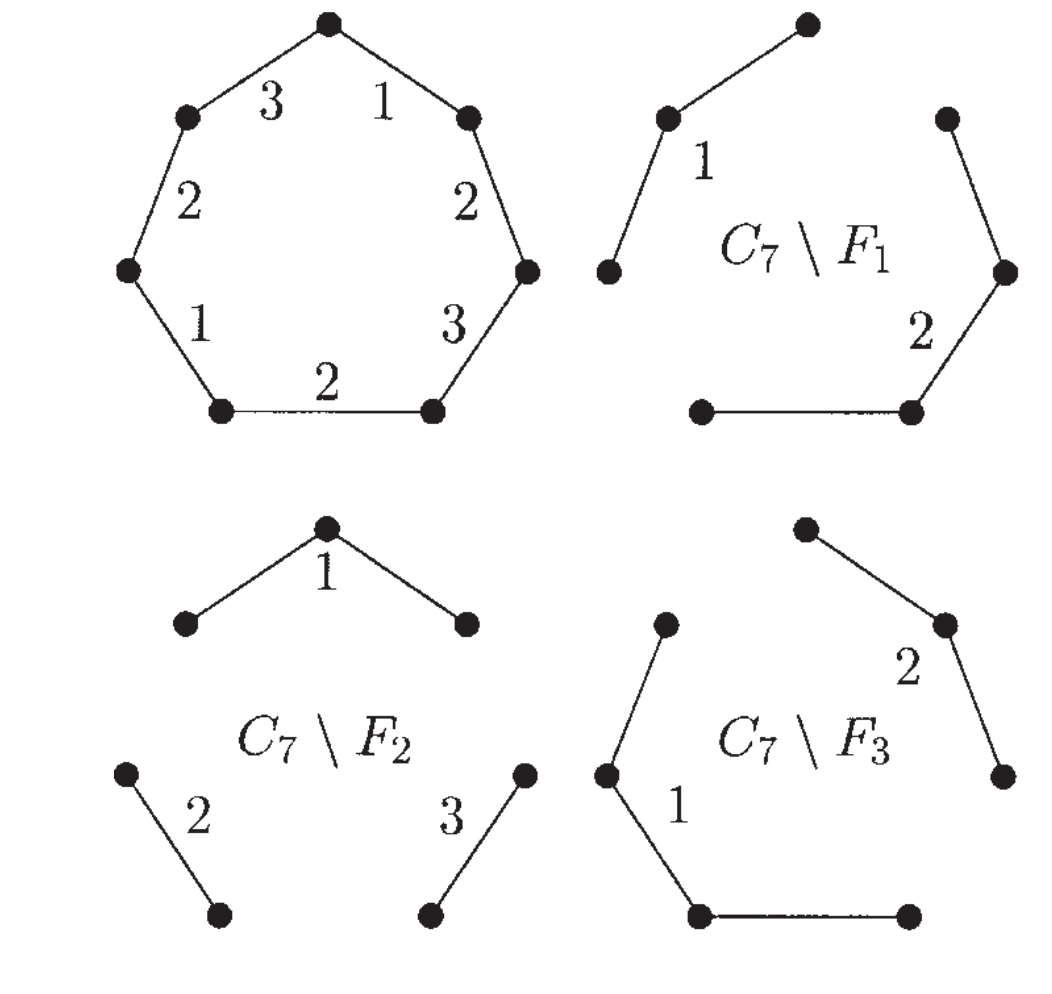
\includegraphics[width=0.8\linewidth]{figures/quotientgraph.png}\label{quotientgraphc7}
\end{center}
\caption{Quotient graph of $C_7$}
\end{figure}
Consider the labeling of the 7-cycle, $C_7$, given in Figure \ref{quotientgraphc7}, and the partition of $E(C_7)$ obtained by defining $F_i$ to be the set of edges labeled $i$, for $i\in \{1,2,3\}$. As we can see, $C_7/ F_1$ and $C_7/F_3$ have only two vertices and since there is an edge in the correspoding $F_i$ connecting those two components, both of  $C_7/ F_1$ and $C_7/F_3$ are simply a $K_2$, while $C_7/ F_2$ has three vertices but each two of compontents are connected with an edge from $F_2$ so $C_7/ F_2$ is simply a $K_3$.   
\newline
Klav\v zar and Peterin defined two conditions in their characterization of induced subgraphs of Hamming graphs. They actually named them by letters $B$ and $C$, and also defined condition A, which was needed for subgraphs of Hamming graphs, but since we will not need condition $A$, we will name the two conditions simply by numbers $1$ and $2$.\newline
We say that a $d$-edge-labeling of $G$ is a ($d$-)KP-labeling if it satisfies the following conditions:
\newline
\textbf{Condition 1} The edges of any triangle have the same label.\newline
\textbf{Condition 2} For any two non-adjacent vertices $u$ and $v$ in $G$, there exist different labels $i$ and $j$ which both appear on any induced $u$, $v$-path.\newline
\begin{figure}[h!]
\begin{center}
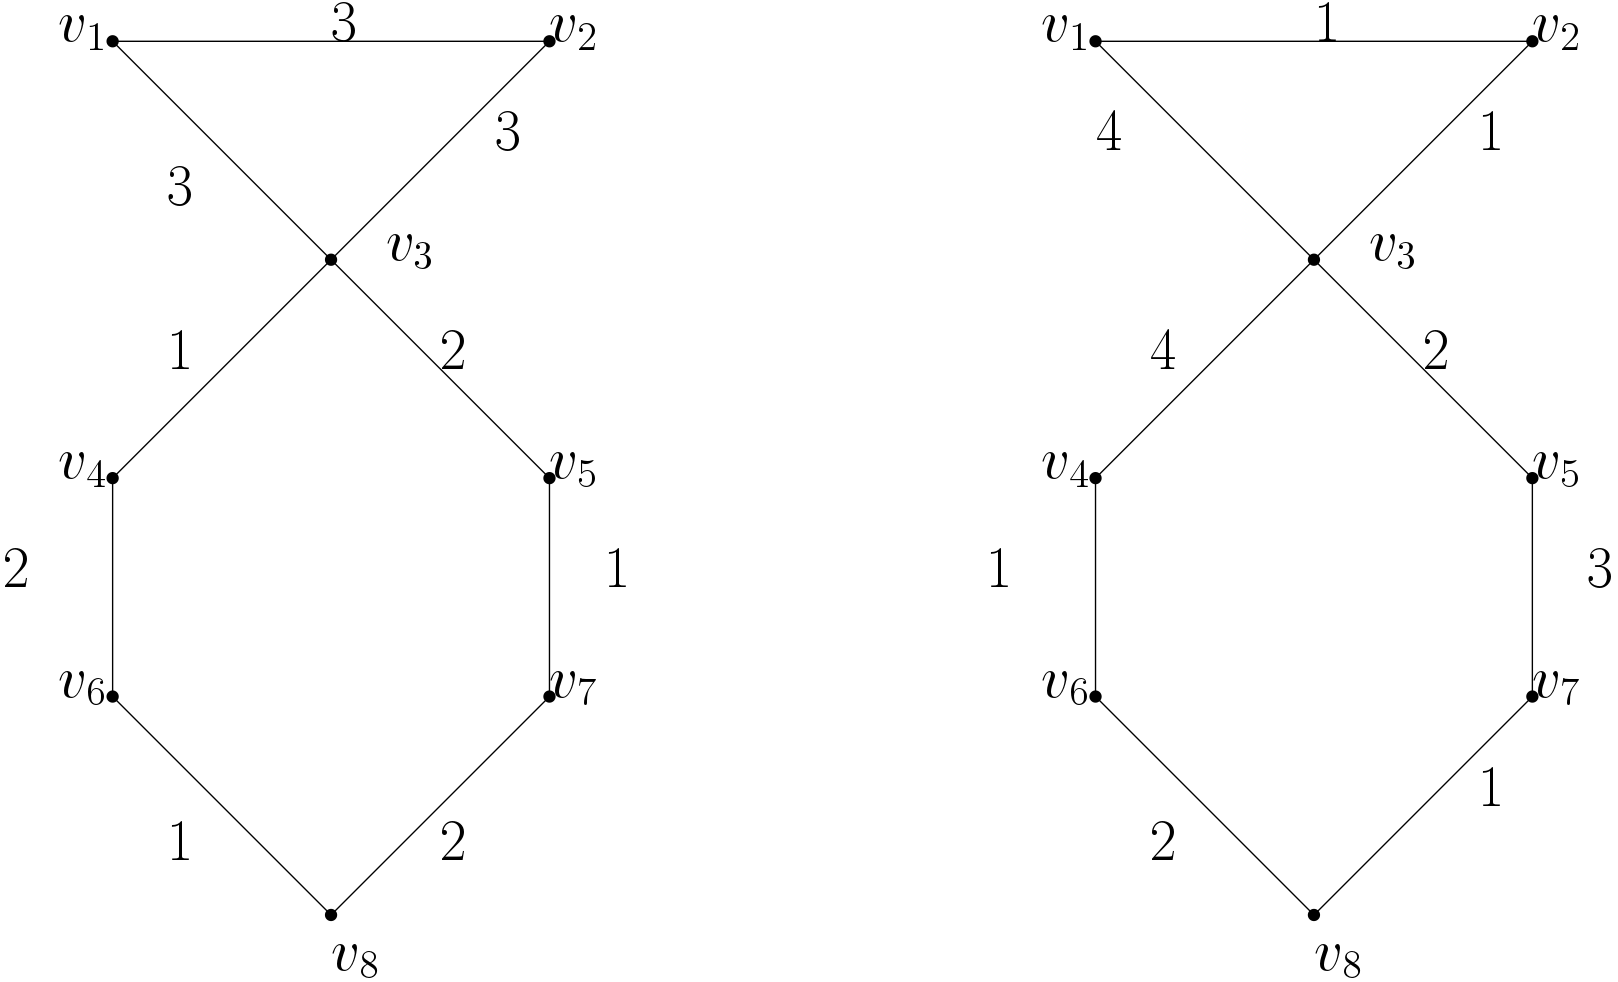
\includegraphics[width=1\linewidth]{figures/kpexample.png}
\end{center}
\caption{The label on the left is a KP-labeling, while the one on the right is not.}\label{kpexample}
\end{figure}
\begin{example}
Let us see two examples of edge labeling of the same graph $G$ as in Figure ~\ref{kpexample}.\newline
The label in the left side of the figure satisfies condition $1$, as the edges of the triangle have the same label. It also satisfies condition $2$, as it can be checked that for arbitrary vertices $u$ and $v$ of $G$ with $d_G(u,v) \geq 2$ there exist different labels $i$ and $j$ which both appear on any induced $u$, $v$-path. Therefore the label in the left side of the figure is a KP-labeling.\newline
The label in the right of the figure satisfies neither condition $1$ nor $2$, as the edges of the triangle do not have the same label, and also if we take vertices $v_5$ and $v_8$ then paths $P_1=v_5v_3v_4v_6v_8$ and $P_2=v_5v_7v_8$ have only one label in their intersection.(Moreover if we consider vertices $v_1$ and $v_4$, then only one label appears on path $v_1v_3v_4$.)
\end{example}
\section{KP-labeling: the definition and basic results}
Examples of graphs with no KP-labeling are $C_5$ and diamon, one can easily show that diamond must be labeled with only one label because of triangles but then Condition 2 will fail.\newline 
Next we try to understand Conditions 1 and 2 on cycle graphs and we infer the following result.
\begin{lemma}\label{lemma:cyclenotunique}Let $G$ be a labeled graph satisfying Condition 2 and let $C$ be an induced cycle in $G$ of length at least 4. Then every label of $C$ is present more than once on $C$.
\end{lemma}
\begin{proof}
The labels of a $u, v$-path of length $2$ on a $C$ must be different, otherwise we cannot find two labels appearing in every $u,v$-path, hence by Condition 2 those two labels should appear also along the other $u,v$-path in $C$. So for any label take two vertices $u$ and $v$ that have distance two and such that a $u,v$-path of length two contains the edge with that label. Then, the label is present on both $u,v$-paths in $C$, therefore the label is present more than once on $C$ 
\end{proof}
In order to prove the main result, we will need also the following lemma.
\begin{lemma}\label{lemma:inducedpaths}Let $G$ be a labeled graph satisfying Conditions 1 and 2 and let $u, v$ be vertices of $G$ with $d_G(u,v)\geq 2$. Then, if labels $i$ and $j$ appear on every induced $u, v$-path, they appear on every $u, v$-path.
\end{lemma}
\begin{proof}
Suppose that labels $i$ and $j$ appear on every induced \textsc{$u, v$}-path but not on every $u, v$-path. Let $P=x_1x_2\ldots x_r$, with $x_1=u$, $x_r=v$, be a $u, v$-path of minimal length that does not contain both labels $i$ and $j$. Then $P$ is not induced since every induced path contains both labels, hence we have an edge between some non-consecutive vertices, say $e=x_kx_l$ with $l-k>1$. We may assume that $e$ is chosen so that $l-k$ is as small as possible. By the minimality of $P$, the path $x_1x_2\ldots x_kx_lx_{l+1}\ldots x_r$ (which is shorter than $P$) contains both labels $i$ and $j$. Hence, the label of the edge $x_kx_l$ is either $i$ or $j$, otherwise $P$ would contain both labels $i$ and $j$. Assume without loss of generality that the label is $i$. Then, label $j$ appears either on the path $x_1x_2...x_k$ or on the path $x_lx_{l+1}...x_r$ (note that it cannot happen that $k=1$ and $l=r$ as $d_G(u,v)\geq 2$). It follows that $i$ does not appear on the path $x_kx_{k+1}...x_l$. But then label $i$ appears only once on the induced cycle $C=x_kx_{k+1}...x_lx_k$. If $C$ is a triangle, we have a contradiction with Condition 1, otherwise with Lemma \ref{lemma:cyclenotunique}.
\end{proof}
If $G$ is a tree, then assigning a different label to each edge results in a labeling satisfying Conditions 1 and 2, hence in a $KP$-labeling. Note that every edge in a tree is a cut-edge. More generally, we can ask: which edges in a graph that has a $KP$-labeling can receive a unique label in some $KP$-labeling? This question is answered by the following result. 
\begin{proposition}
Let $G$ be a graph having a $KP$-labeling and let $e$ be an edge in $G$. Then $G$ has a $KP$-labeling in which $e$ receives a unique label if and only if $e$ is a cut-edge.
\end{proposition}

\begin{proof}
First we will show that if $e$ is a cut-edge then $G$ has a $KP$-labeling in which $e$ receives a unique label. Fix an arbitrary $KP$-labeling of G.\newline
Relabel edge $e$ with a new label, say $i$, not used before. We will show that the new labeling is also a $KP$-labeling. We need to verify the following two conditions:\newline
Condition 1: Every triangle is monochromatic.\newline Condition 1 holds, since $e$ is not part of any cycle (see Lemma \ref{cutedgecycle}) and therefore every triangle is still monochromatic.\newline
Condition 2: for every pair of distinct non-adjacent vertices $u,v$, there exist different labels $j$ and $k$ which both appear on every iduced $u,v$-path.\newline
To verify condition 2, note that any two $u,v$-paths either both contain edge $e$ or none (otherwise $e$ would be part of a cycle, contradicting Lemma \ref{cutedgecycle}).\newline
If none of the induced $u,v$-paths contains edge $e$ then the new $KP$-labeling still satisfies Condition 2 for the pair $u,v$ because of the original $KP$-labeling satisfied the condition for this pair.\newline
Otherwise all induced $u,v$-paths contain $e$. Let the original label of $e$ be $i_0$. Also let $j,k$ be the labels that appear on every $u,v$-path, we consider two cases:
\item[Case 1] If $i_0\in \{j,k\}$ then we take the new label of $e$ and the labeled that appears on every $u,v$-path different from the original label of $e$, more formally $(\{j,k\}\setminus \{i_0\})\cup \{i\}$.
\item[Case 2] If $i_0\not\in \{j,k\}$ then take labels that appeared on every $u,v$-path, more formally $\{j,k\}$.\newline
For the converse direction, suppose $G$ has a $KP$-labeling in which $e$ receives a unique label. Suppose for contradiction that $e$ is not a cut-edge. Then by Lemma \ref{cutedgecycle} $e$ is part of a cycle $C$. If $C$ is a triangle, then by Condition 1 every edge of $C$ must have the same label as $e$, but then $e$ would not be labeled uniquely. Therefore $C$ cannot be triangle. 
Let $V(C) = \{v_1, v_2, \ldots, v_p\}$ in cyclic order and without loss of generality $e = v_1 v_2$. Let $u = v_1$ and $v = v_3$. Vertices $u$ and $v$ are non-adjacent since $e$ is not contained in any triangle. Fix a pair of distinct labels $i$ and $j$ that appear on every induced $u,v$-path (such a pair exists from Condition 2). By the Lemma \ref{lemma:inducedpaths}, labels $i$ and $j$ also appear on the $u,v$-path $v_1v_kv_{k-1}\ldots v_3$, contradicting the assumption that $e$ is labeled uniquely
\end{proof}
\section{Induced subgraphs of Hamming Graphs}
The following characterization of induced subgraphs of Hamming graphs is due to Klav\v zar and Peterin \cite{Iztok}.
\begin{theorem}\label{thm:mainkp}
Let $G$ be a connected graph. Then $G$ is an induced subgraph of a Hamming graph of dimension $d$ if and only if $G$ has a $d$-KP-labeling.
\end{theorem}
\begin{proof}
Let $G$ be an induced subgraph of $H=K_{n_1}\square K_{n_2}\square\cdots\square K_{n_d}$. To make things easier denote $p_i=p_{K_{n_i}}$, which is the projection to the complete graph $K_{n_i}$ of $H$ and also consider the labeling $E(G)$ induced by the color map $c$ of $H$. We will show that this labeling satisfies Conditions $1$ and $2$.\newline
Condition $1$ is clear. Indeed, if $u$, $v$, and $w$ induce a triangle, then they all lie in
the same layer of $H$ and by the alternative description of Hamming graphs we have that each pair is adjacent so they differ in exactly in one coordinate. Therefore color map $c$ will map those edges to the coordinate in which they differ and so the edges $uv$, $uw$, and $vw$ receive the same label.\newline
We next show that Condition $2$ is satisfied, too. Let $u$ and $v$ be two vertices of $G$ with $d_G(u,v)\geq 2$.
Suppose that there is no label that appears on all induced $u, v$-paths. Now if we see $u$ and $v$ as $d$-tuples and we understand walking along paths as changing coordinates. Therefore $p_i(u)=p_i(v)$ for all $i$ because if we look at one induced $u,v$-path that does not have label $i$, that means than we never change the $i^{th}$ coordinate as we traverse this path and therefore the $i^{th}$ coordinates are the same. This implies $u=v$, contrary to $d_G(u,v)\geq 2$. Suppose now that all induced $u, v$-paths have exactly one label in common, say $i$. We have $p_j(u)=p_j(v)$ for all $j\neq i$ and consequently $p_i(u)\neq p_i(v)$ (since $u\neq v$). Vertices $p_i(u)$ and $p_i(v)$ are adjacent in $K_{n_i}$, since $K_{n_i}$ is a complete graph. Hence, $u$ and $v$ are adjacent in $H$ and therefore also in $G$, which is impossible, since $d_G(u,v)\geq 2$.\medskip \newline 
Conversely, let $\ell$ be a $d$-edge-labeling of $G$ that fulfills Conditions 1 and 2. Let $\mathcal{F}=\{F_1,F_2,\ldots F_d\}$ be the partition of $E(G)$ induced by $\ell$ and let $f$ be the quotient map of $G$ with respect to $\mathcal{F}$. We claim that $f$ embeds $G$ as an induced subgraph into $G=(G/ F_1)\square (G/ F_2)\square \ldots \square (G/ F_d)$.\newline
We show first that $f$ is one-to-one. Suppose that vertices $x$ and $y$ are not adjacent in $G$. Then by Condition 2 and Lemma ~\ref{lemma:inducedpaths}, there exist labels $i$ and $j$ such that on every $x, y$-path in $G$ we find labels $i$ and $j$. So $x$ and $y$ are in different components in both $G\backslash F_i$ and $G\backslash F_j$. Already the first fact assures that $f(x)\neq f(y)$. Let next $x$ and $y$ be adjacent vertices of $G$ and let $l(xy)=i$. We can see that $f_j(x)=f_j(y)$ for every $j\neq i$, vertices $x$ and $y$ belong to same component $G-F_j$ as they are adjacent.

 Now let us take a look at $f_i$. Suppose that there exists an $x, y$-path $P=x_1x_2\ldots x_r$ in $G\backslash F_i$, where $x_1=x$ and $x_r=y$. We can assume that $P$ is shortest among all $x, y$-paths in $G\backslash F_i$. If $P$ is induced in $G-xy$ we have a contradiction with Condition 1 when $r=3$ since $P$ does not contain label $i$ (recall that $P$ is in $G\backslash F_i$) but a triangle will be formed with $xy$ and two edges in $P$. When $r>3$, we have a contradiction with Lemma ~\ref{lemma:cyclenotunique} if $P$ is an induced path in $G-xy$ because $P+xy$ would form a cycle in which label $i$  is present only once. Thus $P$ is not induced in $G-xy$, $r > 3$, and there are adjacent vertices $x_j$ and $x_k$ with $k > j+1$ and $\{j,k\}\neq \{1,r\}$. By the minimality of $P$ we have $\ell(x_jx_k)=i$. We can select $j$ and $k$ such that $k- j$ is minimal among all such vertices $x_j$ and $x_k$. Then the cycle $C=x_jx_{j+1}\ldots x_{k-1}x_k$ is induced. If $C$ is a triangle we have a contradiction with Condition 1, otherwise we have a
contradiction with Lemma ~\ref{lemma:cyclenotunique}. Hence, $f_i(x)\neq f_i(y)$ and we have shown that $f$ is one-to-one.\newline
Let $xy$ be an edge of $G$ with $\ell(xy)=i$. Then, by the above, $x$ and $y$ are in different components of $G\backslash F_i$. Moreover, they belong to the same component in any of the graphs $G\backslash F_j$ , for $j\neq i$. It follows that $f$ maps edges to edges.\newline
Let $x$ and $y$ be non-adjacent vertices of $G$. Then, by the same reasoning as above, $x$ and $y$ are in different components of at least two graphs $G\backslash F_i$. It follows that $f(x)$ and $f(y)$ differ in at least two coordinates and this fact remains valid after adding edges to the factor graphs. It follows that $f$ maps non-edges to non-edges and the claim is proved.\newline
Hence, $G$ is isomorphic to the subgraph $G\backslash F_1\square G\backslash F_2\square \ldots \square G\backslash F_k$ induced by $f(V(G))$. To complete the proof we show that $G$ is also an induced subgraph of the Hamming graph $K_{|V(G\backslash F_1)|}\square K_{|V(G\backslash F_2)|}\square \ldots \square K_{|V(G\backslash F_k)|}$ : 
\end{proof}
\begin{example} Let us see that $C_7$ is an induced subgraph of a Hamming graph by showing that there exists a labeling of $C_7$ that fulfills Conditions $1$ and $2$.
\begin{figure}[h!]
\begin{center}
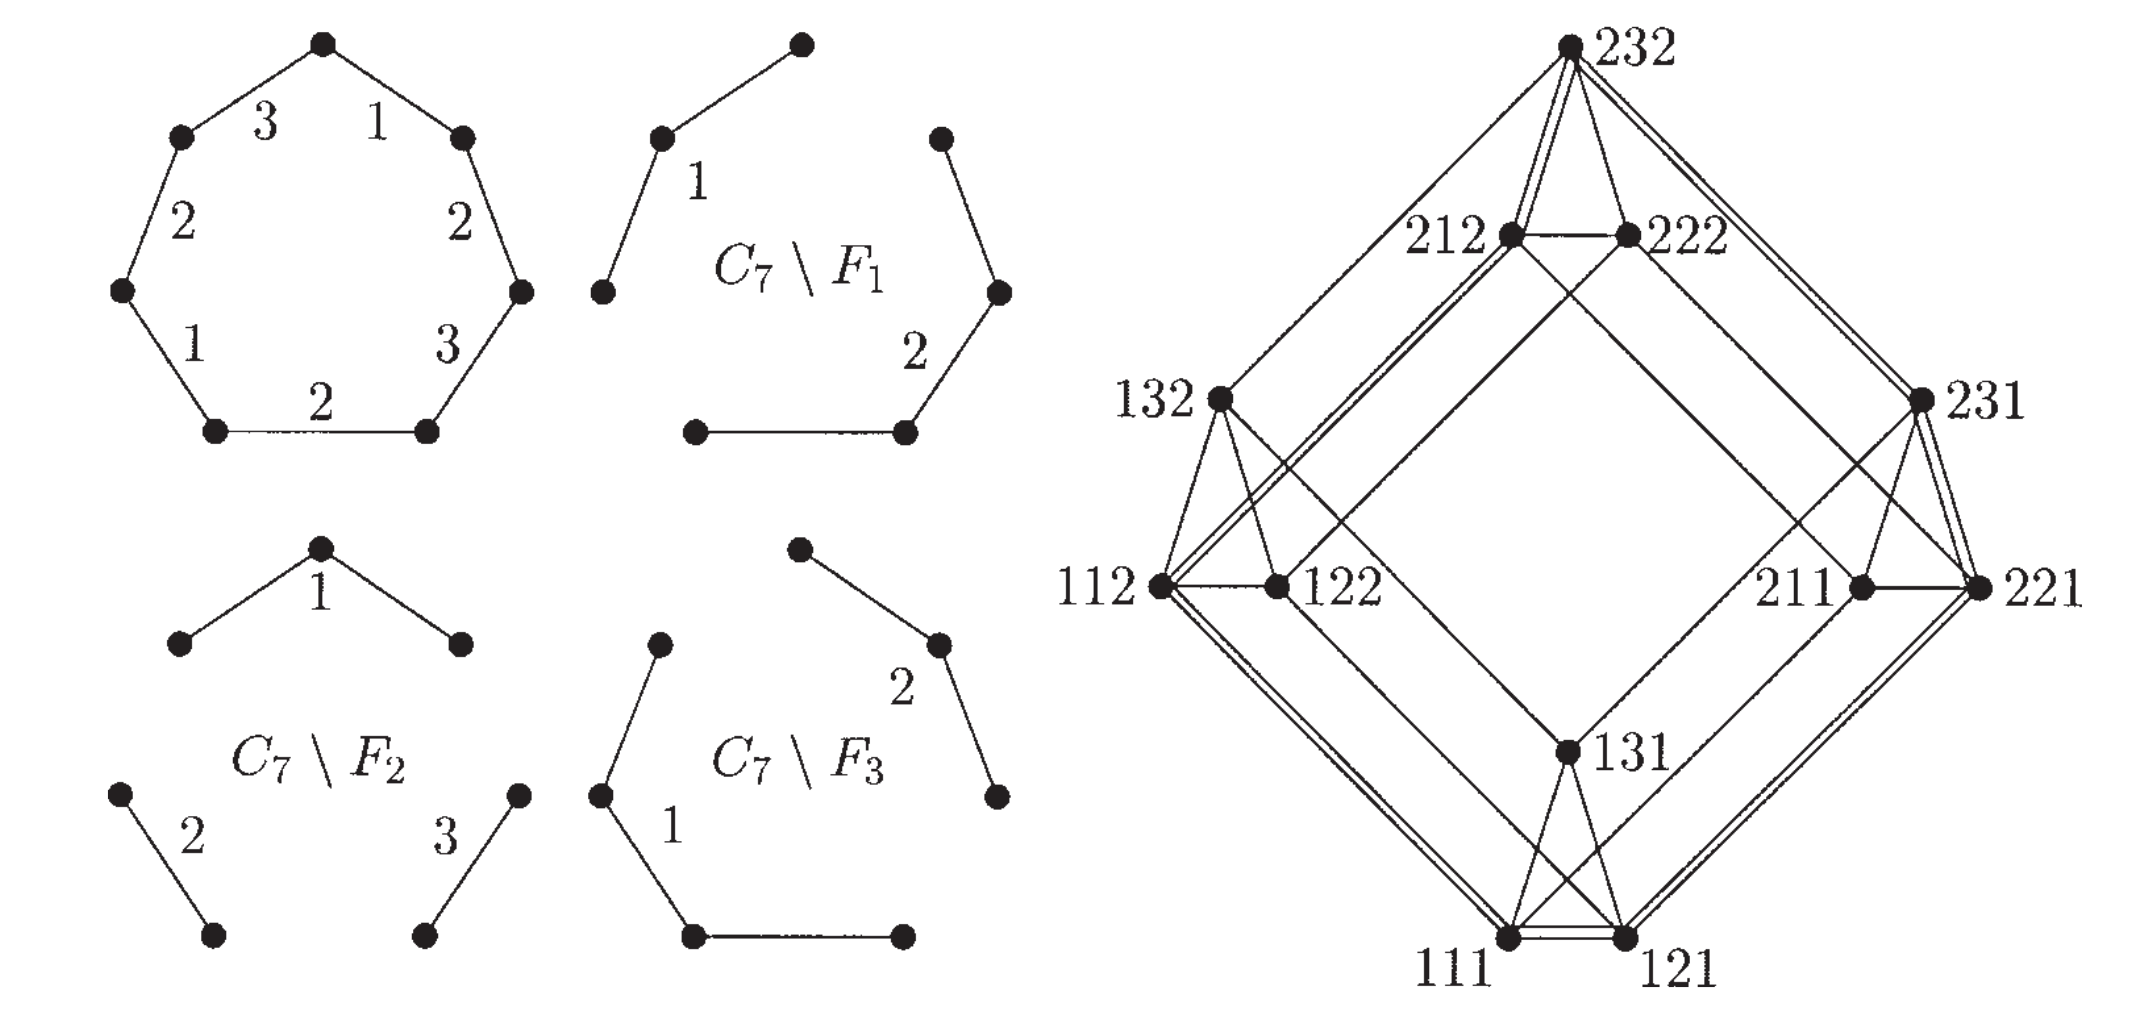
\includegraphics[width=0.8\linewidth]{figures/c_7inducedhamming.png}
\end{center}
\caption{$C_7$ as an induced subgraph of $K_2\square K_3\square K_2$.}\label{fig:c7induced}
\end{figure}
\newline
$C_7$ is an induced subgraph of $K_2\square K_3\square K_2$. In Figure \ref{fig:c7induced} take the cycle $(112,212,232,231,221,121,111)$ and using the color map $c$, edge $\{111,112\}$ gets label $3$, edge $\{112,212\}$ gets label $1$, and edge $\{212,232\}$ gets label $2$, edge $\{232,231\}$ gets label $3$, edge $\{231,221\}$ gets label $2$, edge $\{221,121\}$ gets label $1$, and edge $\{121,111\}$ gets label $2$. We can easily check that edges of a triangle have the same label (here there is no triangle, which is fine) and for any two vertices $u$ and $v$ of $C_7$ with $d_{C_7}(u,v) \geq 2$, there exist different labels $i$ and $j$ which both appear on any induced $u, v$-path.\newline
$C_7$ has a labeling in which Conditions 1 and 2 hold as the first graph in Figure ~\ref{fig:c7induced}. Now let us take a look at where does the map $f$ send vertices of $C_7$. We follow the order clockwise from top-most vertex $f$ maps the first vertex to $112$, the second vertex to $212$, the third vertex to $232$, the fourth vertex to $231$, the fifth vertex to $221$, sixth vertex to $121$, and the seventh vertex to $111$. As we can see $G\cong f(G)$ and an induced subgraph of $K_2\square K_3\square K_2$.
\end{example}
Note that the quotient graphs obtained in the proof of Theorem \ref{thm:mainkp} need not be complete. For instance, consider the path $P_4$ together with the labeling 1, 2, 1 along the edges of the path (in order). Then get $G/ F_1\cong P_3$.
\chapter{Cartesian dimension}\label{cdim-chapter}
Given a positive integer $d$, a $d$-realization of a graph $G=(V,E)$ is an injective mapping $\varphi_G:V\to \mathbb{R}^d$ such that two vertices $u, v \in V$ are adjacent if and only if $\varphi_G(u)$ and $\varphi_G(v)$ differ in exactly one coordinate. A graph $G$ is said to be $d$-realizable if it has a $d$-realization. Note that $G$ is $d$-realizable if and only if $G$ has a $d$-realization $\varphi_G : V \rightarrow \mathbb{N}^d$ or a $d$-realization $\varphi_G:V\to S^d$ where $S\subseteq \mathbb{N}$ is sufficiently large, since $V(G)$ is finite.\newline
Any graph that has a $d$-realization, also has a $(d+1)$-realization (simply add one coordinate constantly equal to $0$). This naturally leads to a definition: the Cartesian dimension of a graph $G = (V, E)$, denoted $Cdim(G)$, is defined as the minimum non-negative integer $d$ such that $G$ is $d$-realizable, if such an integer exists, and $\infty$, otherwise. Note that $K_1$ is the only graph of Cartesian dimension 0.\newline

For a graph $G$ to have Cartesian dimension $1$ it must have a $1$-realization, or, in other words, we can map all the vertices of the graph to $\mathbb{R}$. Becuase the map has to be injective, every vertex is mapped to different a real number. But then every two vertices differ in exactly one coordinate, which makes them adjacent. Therefore the only graphs of Cartesian dimension $1$ are exactly the complete graphs of order at least $2$.

\begin{example}
$C_6$ has Cartesian dimension $2$. Indeed, since it is not a complete graph it cannot have dimension $1$, and we find a $2$-realization of $C_6$ with vertex set $V=\{v_1,v_2,v_3,v_4,v_5,v_6\}$ and edge set $E=\{v_1v_2,v_2v_3,v_3v_4,v_4v_5,v_5v_6,v_6v_1\}$ by the map $\varphi_{C_7}:V\to \mathbb{R}^2$ given by $\varphi(v_1)=(1,1)$, $\varphi(v_2)=(3,1)$, $\varphi(v_3)=(3,3)$, $\varphi(v_4)=(2,3)$, $\varphi(v_5)=(2,2)$, and $\varphi(v_6)=(1,2)$ (see Figure \ref{c_62real}). An easy check shows that indeed for any edge the corresponding values of $\varphi$ differ in exactly one coordinate, while for any non-edge they differ in both coordinate.
\begin{figure}[h]
\begin{center}
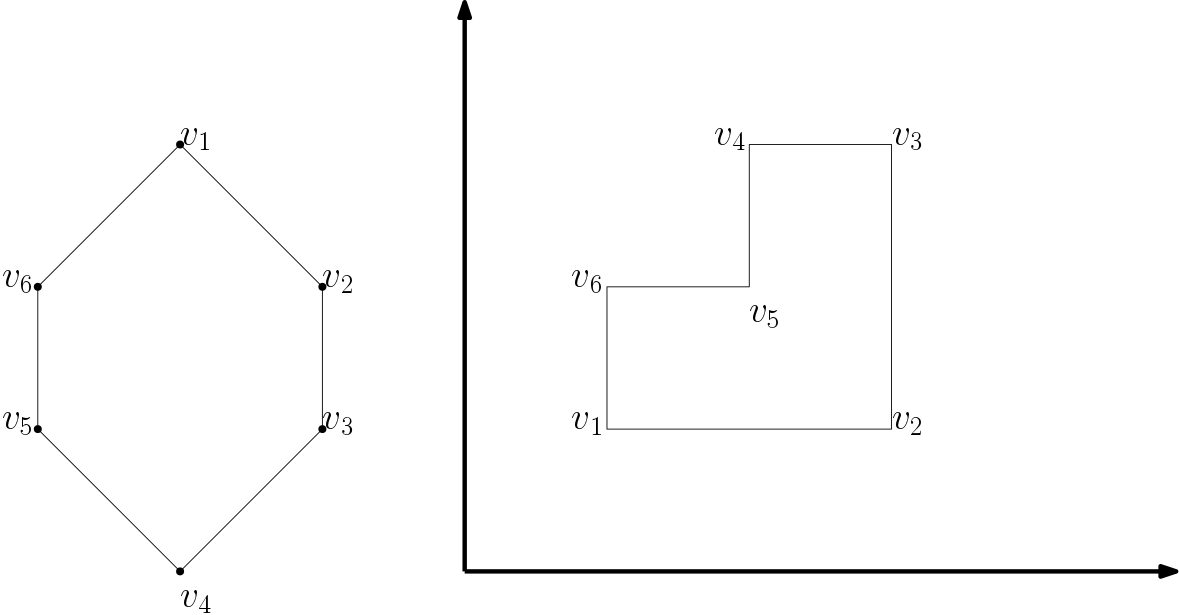
\includegraphics[width=1\linewidth]{figures/c_62real.png}
\end{center}
\caption{A $2$-realization of $C_6$}\label{c_62real}
\end{figure}
\end{example} 
We will see that diamond-free graphs may have $2$-realization, and to show that we first need the following lemma:  
\begin{lemma}\label{diamondfreecliques}
If a graph $G$ is diamond-free then any two maximal cliques of $G$ intersect in at most one vertex.
\end{lemma}
\begin{proof}
Suppose two maximal cliques $A_1$ and $A_2$ intersect in at least two vertices, say $v_1, v_2$. Let $v_3$ be a vertex in $A_1$ non-adjacent to some vertex $v_4\in A_2$(such a pair of vertices exists since otherwise $A_1\cup A_2$ would be a clique). But then vertices $v_1,v_2,v_3,v_4$ induce a diamond, a contradiction with $G$ being diamond-free.
\end{proof}

\begin{theorem}[Staton and Wingard~\cite{Staton}]
For every graph G, the following conditions are equivalent:
\begin{enumerate}
\item $Cdim(G)\leq 2$.
\item $G$ is the line graph of a bipartite graph.
\item $G$ is diamond-free and its clique graph $K(G)$ is bipartite.
\item $G$ is \{claw, diamond, $C_5$, $C_7$, \ldots\}-free.
\end{enumerate}
\end{theorem}

\begin{proof}\sloppypar
First, we prove that condition 1 implies condition 4. We show that none of the graphs in condition 4 can be an induced subgraph of a graph with $Cdim(G)\leq 2$. Suppose that $G$ is not \{claw, diamond, $C_5$, $C_7$, \ldots\}-free, $Cdim(G)$ cannot be equal to $1$ since only complete graphs have Cartesian dimension $1$. Now suppose that $Cdim(G)=2$.
\newline First let us consider the diamond. Suppose $G$ has a diamond graph, H as induced subgraph with vertex set $V(H)=\{v_1,v_2,v_3,v_4\}$ and edge set $E(H)=\{v_1v_2,v_1v_3,v_2v_3,v_2v_4,v_3v_4\}$. Now because $v_1$, $v_2$, and $v_3$ induce a complete graph on $3$ vertices, all three together differ in the same coordinate, similarly for $v_2$, $v_3$ and $v_4$. It follows that also $v_1$ and $v_4$ differ only in one coordinate but they are not adjacent, a contradiction.
\newline Next suppose $G$ has a claw graph, $H$, as induced subgraph with vertex set $V(H)=\{v_1,v_2,v_3,v_4\}$ and edge set $E(H)=\{v_1v_2,v_1v_3,v_1v_4\}$. Without loss of generality assume that $\varphi_G(v_1)$ differs only in the first coordinate with $\varphi_G(v_2)$. Because $v_2$ and $v_3$ are not adjacent, $\varphi_G(v_1)$ and $\varphi_G(v_3)$ must differ only in the second coordinate. Because $v_1$ and $v_4$ are adjacent, they must differ in only one coordinate, but either coordinate is not good as that would  imply adjacency between $v_4$ and $v_2$, or between $v_4$ and $v_3$, but there is no edge among them.
\newline Finally, consider ann odd cycle of length more than 3. Let the vertex set be $V(H)=\{v_1,v_2,\ldots,v_k\}$ with edge set $E(H)=\{v_1v_2,v_2v_3,\ldots ,v_kv_1\}$ and notice that since there is no triangle, no three vertices lie in the same line so if we consider the color map define in Section ~\ref{kp-labeling-section} then by following the cycle we must alternate by colors $1$ and $2$, but the cycle is odd, so is not possible.\newline
Now, we prove that condition 4 implies condition 3.\medskip \newline Suppose that $G$ is $\{claw, diamond, C_5, C_7, \ldots \}$-free. We only need to show that $K(G)$ is bipartite, which is equivalent to showing that $K(G)$ has no odd cycle. Suppose $K(G)$ has an odd cycle of length greater than $3$. First note that no three  maximal cliques (vertices in $K(G)$) share one vertex as then a claw would be formed in $G$ (see Appendix) but $G$ is claw-free. 

Thus we form an odd cycle in $G$ by following the common vertices of cliques of size greater than $3$. But $G$ is $\{C_5,C_7,\ldots\}$-free, therefore $K(G)$ has a cycle of length $3$. Let those cliques that form a triangle be $A_1,A_2,A_3$ and the common vertex of $A_1$ and $A_2$ is $v_1$; the common vertex of $A_2$ and $A_3$ is $v_2$; whereas the common vertex of $A_3,A_1$ is $v_3$, because $v_1$ and $v_2$ are in $A_2$ they are adjacent, similiarly for others. Vertex $v_3$ is not in $A_2$ but has two neighbors in $A_2$ ($v_1$ and $v_2$), contradiction with Corollary TODO in Appendix A. Therefore $K(G)$ is bipartite.\newline \medskip 
Now let us show that condition 3 implies condition 1. If $G$ is complete then we know that $Cdim(G)=1$. Suppose that $G$ is not complete. Since $K(G)$ is bipartite, we can properly color the vertices of $K(G)$ with two colors. Map the vertices of $G$ in $\mathbb{R}^2$ by placing cliques of $G$ having one color on distinct vertical lines and cliques having the other color on distinct horizontal lines. By Lemma~\ref{diamondfreecliques}, no two vertices are mapped to same point. This gies a 2-realization of $G$, showing that $Cdim(G)\leq 2$.
\newline
Now let us show that condition 1 holds if and only if condition 2 holds. $G$ is the line graph of a bipartite graph, say $H$, in other words $L(H)=G$. Order the vertices of $H$ in any way and construct the adjacency matrix $A$ of $H$. Mark points in $\mathbb{R}^2$ at $(i, j)$ if and only if $i<j$ and $a_{ij} = 1$. 

It is immediate that one can map vertex $\{i,j\}\in V(G)$ to $(i,j)$ where $i<j$ and notice that this defines a one-to-one mapping and if two vertices are adjacent in $G$ then they will differ in exactly on coordinate, this mapping works only if H is bipartite becasuse otherwise H would have an odd cycle and line graph of $H$ would also have an odd cycle which is not possible from implication 4. This shows that $Cdim(G)\leq 2$ as we found a $2$-realization.\newline
Since $G$ can be realized with vertices only at positive integral points (the map $\varphi_G$ can be defined to map to $\mathbb{N}^d$), the proof works in reverse by constructing the adjacency matrix which would lead that $G$ is the line graph of a bipartite graph.
\end{proof}
We move on to understand when a graph is $d$-realiable, first let us answer the question if in a $d$-realizable graph, if a vertex is adjacent to two other vertices, are those two adjacent?
\begin{lemma}\label{xyv adjacent}
Let $G$ be a $d$-realizable graph. Let $v$ be a vertex adjacent to vertices $x$ and $y$. Then $x$ and $y$ are adjacent if and only if both of them differ from $v$ in the same coordinate, and assume we have the $d$-realization $\varphi_G$.
\end{lemma}
\begin{proof}
($\implies$) If $x$ and $y$ are adjacent then $\varphi_G(x)$ and $\varphi_G(y)$ differ in exactly one coordinate say in $k$th coordinate. Also say $\varphi_G(v)$ differs from $\varphi_G(x)$ exactly in the $i$th coordinate and from $\varphi_G(y)$ in the $j$th coordinate. Now suppose $x$ and $y$ do not differ from $v$ in the same coordinate, which means that $i\neq j$, also note that $k$ cannot be equal to both $i$ and $j$ as this would imply $i=j$ so w.l.o.g. $k\neq j$. 

Now because $i\neq j$, the $j$th coordinate of $x$ is the same as the $j$th coordinate of $v$ and therefore differs from $j$th coordinate of $y$, but also $k\neq j$ which means that $x$ and $y$ differ in more than one coordinate. This contradicts the fact that $x$ and $y$ are adjacent.\newline
($\impliedby$) If $x$ and $y$ differ from $v$ in the same coordinate and because both of them are adjacent to $v$ then it means that they differ in exactly that coordinate in which they differ with $v$, i.e., in one coordinate. Therefore they are adjacent.
\end{proof}

\begin{theorem}\label{d-realizable-free}
For every non-negative integer $d$, d-realizable graph is \{$K_{1,d+1}$, diamond,
$K_{2,3}$, $C_5$ \}-free.
\end{theorem} 
\begin{proof} Let $G$ be a $d$-realizable graph, and $\varphi_G$ be the $d$-realization of $G$.\newline
\textit{For $K_{1,d+1}:$} Suppose $v$ is the hub (the vertex with largest degree) of an induced $K_{1,d+1}$ in $G$. Then $\varphi_G(v)$ differs from $d+1$ neighbors in different coordinates by Lemma \ref{xyv adjacent}, but there are only $d$ coordinates, a contradiction.\newline
\textit{For the diamond:} If $v_1$, $v_2$, $x$ and $y$ are vertices of an induced diamond with $v_1$ and $v_2$ the vertices of degree $2$, then, invoking Lemma \ref{xyv adjacent} we see that $\varphi_G(v_1)$ differs from $\varphi_G(x)$ and $\varphi_G(y)$ in the same coordinate. Similarly $\varphi_G(v_2)$ difers from $\varphi_G(x)$ and $\varphi_G(y)$ in the same coordinate.

 Hence $v_1$ and $v_2$ differ from $x$ and $y$ in the same coordinate, and thus either $x=y$ or $x$ is adjacent to $y$, a contradiction.\newline
\textit{For $K_{2,3}$:} Let $x$ and $y$ be adjacent to all $v_1$,$v_2$,$v_3$ in an induced $K_{2,3}$. Then by Lemma ~\ref{xyv adjacent}, $\varphi_G(v_1)$,$\varphi_G(v_2)$, $\varphi_G(v_3)$ differ from $\varphi_G(x)$ in $3$ distinct coordinates. 

We may assume that all coordinate values of $\varphi_G(x)$ are zeros. Then $\varphi_G(y)$ is at a distance of $2$ from $\varphi_G(x)$, so $\varphi_G(y)$ has exactly $2$ non-zero coordinates. Hence $\varphi_G(y)$ has a zero in coordinate where either $\varphi_G(v_1)$, $\varphi_G(v_2)$ or $\varphi_G(v_3)$ is non-zero, and it follows that $y$ differs from one of these $3$ vertices in $3$ coordinates, and is therefore not adjacent to that vertex.\newline
\textit{For the $C_5$:} Let $v_1$,$v_2$,$v_3$,$v_4$,$v_5$ be the vertices of a $5$-cycle in cyclic order. We assume that the coordinates of $\varphi_G(v_1)$ are all zeros.
$$\varphi (v_1)=(0,0,0,\ldots)$$ where $\varphi$ is the map from vertex set to $\mathbb{R}^d$.\newline
Without loss of generality we can say
$$\varphi (v_2)=(\alpha,0,0,\ldots) \text{, for some } \alpha \in \mathbb{R} $$
By the Lemma \ref{xyv adjacent} without loss of generality
$$\varphi (v_3)=(\alpha,\beta,0,0,\ldots) \text{, for some } \beta \in \mathbb{R}$$
Now if $v_4$ differed from $v_3$ in any coordinate other than the first two, $v_4$ would be at a distance at least $3$ from $v_1$ and it would be impossible to find $v_5$ to complete the $5$-cycle. Hence $v_4$ differs from $v_3$ in one of the first 2 coordinates. If 
$$\varphi (v_4)=(\alpha,\gamma,0,0,\ldots) \text{, for some } \gamma \in \mathbb{R}$$
then $v_4$ is adjacent to $v_2$. Hence
$$\varphi (v_4)=(\delta,\beta,0,0,\ldots) \text{, for some } \delta \in \mathbb{R}$$
and the only choice for $v_5$ are
$$(\delta,0,0,0,\ldots)$$
and 
$$(0,\beta,0,0,\ldots)$$
In the first case $v_5$ is adjacent to $v_2$, and, in the  second one, to $v_3$; a contradiction.
 
\end{proof}
\medskip
We take a closer look at the 3-dimensional case and present two results. Both are related to the Klav\v zar-Peterin characterization which is needed for hardness proof for recognizing 3-realizable graphs developed in paper \cite{Milanic}.\newline
In the first result, we will see that the defining properties of a 3-KP-labeling are satisfied for a graph as soon as they are satisfied for the family of all its induced subgraphs isomorphic to a cycle or to a $P_3$.

\begin{theorem}\label{3-edge-label}
Let $G$ be a graph. A 3-edge-labeling of $G$ is a KP-labeling if and only if it satisfies the following two conditions:\newline
\textbf{Condition 3}: For every induced cycle $C$ of $G$, the restriction of the labeling to $E(C)$ is
a KP-labeling of $C$.\newline
\textbf{Condition 4}: No induced $P_3$ is monochromatic.
\end{theorem}

\begin{proof}
Let us start by showing the necessity of the two conditions. If $G$ is 3-KP-labeling and $H$ is an induced subgraph of $G$, then the restriction of the labeling to $E(H)$ is a 3-KP-labeling of $H$ because Conditions 1 and 2 can be easily verified to still hold. Hence Condition 3 is necessary. Condition 4 follows from the fact that every induced $P_3$, say $v_1$, $v_2$, $v_3$, must contain two different labels since otherwise Condition 2 would be violated for $v_1$ and $v_3$ in $G$.\newline\medskip 
Now we prove sufficiency. For Condition 1 we need to show that every triangle is monochromatic but from Condition 3 we know that for every induced triangle of $G$, the restriction to edges, which is the same triangle is a KP-labeling, but a triangle is KP-labeled if and only if it is monochromatic.\newline
Now let us show that Condition 2 also holds by contradiction.\newline
Suppose  that there is a 3-edge-labeling $l:E(G)\rightarrow \{1,2,3\}$ satisfying Conditions 3 and 4, but not Condition 2. Singe Condition 2 does not hold in $G$, it means that $G$ contains two different induced paths of length at least two, say $P$ and $Q$, intersecting at their endpoints $u$ and $v$, such that no pair of different labels appears on both $P$ and $Q$.\newline
Due to Condition 4, on each of the paths $P$ and $Q$ at least two different labels appear. Since no pair of different labels appears on both $P$ and $Q$, we may assume that $P$ and $Q$ take alternatingly labels 1, 2 and 1, 3, respectively. Moreover, assume that $P$ and $Q$ were chosen so as to minimize $|V(P)|+|V(Q)|$.\newline
We continue with a definition to facilitate our way in the proof. Given a path $R$ and two of its vertices $x$ and $y$, denote by $R_{xy}$ the subpath of $R$ between
$x$ and $y$, and by $V_R^{-xy}$ the set $V(R)\backslash \{x,y\}$. Also, say a path is $k$-labeled if exactly $k$
different labels appear on its edges.\newline
We claim that $V_P^{-uv} \cap V_Q^{-uv} = \emptyset$. Suppose that there is something in the intersection, say $w\in V_P^{-uv} \cap V_Q^{-uv}$. First we see that $P_{uw}$ and $Q_{uw}$ cannot be 1-labeled since otherwise because of Condition 4 none of the paths can have length more than 2, from which it must follow that $u$ and $w$ are adjacent, but this is in contradiction with minimality of $|V(P)|+|V(Q)|$. 

So it must be that $P_{uw}$ and $Q_{uw}$ are 2-labeled. Since there are only 3 labels, it must be the case that $P_{uw}\cup Q_{uw}$ would be 3-labeled, which is again a contradiction with the minimality of $|V(P)|+|V(Q)|$. \newline
We add also some futher definitions. For $t \in \{u, v\}$ and $xy \in E(G)$ with $(x, y) \in V_P^{-uv} \times V_Q^{-uv}$, a cycle $C = P_{tx}-xy-Q_{yt}$ such that either $P_{tx}-xy$ or $xy-Q_{yt}$ is an induced path will be called a $PQ$-cycle. 

Note that a $P Q$-cycle cannot be 3-labeled: if, without loss of generality say $P' = P_{tx} -xy$ was an induced path, then we can find a shorter pair of paths, namely $P'$ and $Q_{yt}$, which would contradict the minimality of $|V(P)|+|V(Q)|$.\newline
Let us investigate the cycle $C_0=P\cup Q$. From our assumption that no two labels appear in both paths $P,Q$, from Condition 3 we have on induced cycles, the restriction of the labeling to $E(C_0)$ is a KP-labeling of $C_0$ it must follow that $C_0$ is not an induced cycle as the restriction of the labeling to $E(C_0)$ is obviously not a KP-labeling of $C_0$. Let $xy$ be a chord in $C_0$ such that $\{x, y\} \cap \{u, v\} = \emptyset$ and such that $x \in V (P )$ is closest to $u$ (where the distance is measured within $P$), and $y$ is the neighbor of $x$ in $Q$ closest to $v$ (where the distance is measured within $Q$).

 Now we observe two cycles that are formed, namely $C_1 = P_{ux}-xy-Q_{yu}$ and $C_2 = P_{vx} -xy-Q_{yv}$. Because of how we selected $x$ and $y$ each of $C_1,C_2$ is either a $P Q$-cycle or a triangle, implying that neither of them is 3-labeled. If $C_1$ is monochromatic, then, as $E(C_0) \subset E(C_1 ) \cup E(C_2)$ while $C_1$ and $C_2$ share the label of $xy$, it would follow that $C_2$ was 3-labeled, symmetricaly if $C_2$ was monochromatic. Thus, $C_1$ and $C_2$ are 2-labeled. \newline
As $C_1$ and $C_2$ are 2-labeled, they share exactly one label. By definition, any $P Q$-cycle contains a $P_3$ from either $P$ or $Q$, hence (recalling that $P$ and $Q$ alternate labels 1, 2 and 1, 3, respectively), $C_1$ and $C_2$ share label 1. Such is then the label of $xy$. However, one of the two edges incident to $x$ in $P$ is also labeled with 1, forming with $xy$ a monochromatic
induced $P_3$ (as part of either $C_1$ or $C_2$), which contradicts Condition~4. 
\end{proof}

\begin{example}
We will see an example showing that a statement analogous to Theorem \ref{3-edge-label} does not work for 4-edge-labelings. We find a labeled graph satisfying Conditions 3 and 4 that is not KP-labeled.\newline
Take the graph $G$ with 4 paths of length 6 sharing only the endpoint vertices, say $u$ and $v$. Label the paths in following way:\newline
\textit{path 1: 1, 2, 3, 1, 2, 3}\newline
\textit{path 2: 2, 3, 4, 2, 3, 4}\newline
\textit{path 3: 3, 4, 1, 3, 4, 1}\newline
\textit{path 4: 4, 1, 2, 4, 1, 2}\newline
A quick check can show that every induced cycle is KP-labeled and also no $P_3$ is monochromatic, which means that Conditions 3 and 4 are satisfied. 

However if we check whether this labeling is a KP-labeling of $G$, taking non-adjacent vertices $u$ and $v$, we can see that each pair of the 4 paths share exactly 2 labels, but from pingeonhole principle we cannot find labels $i$ and $j$ which both appear on any induced $u, v$-path.\newline
This example can be generalized to show an analogue of that Theorem \ref{3-edge-label} does not work for $d$-labeling for any $d>3$.  
\begin{figure}[h]
\begin{center}
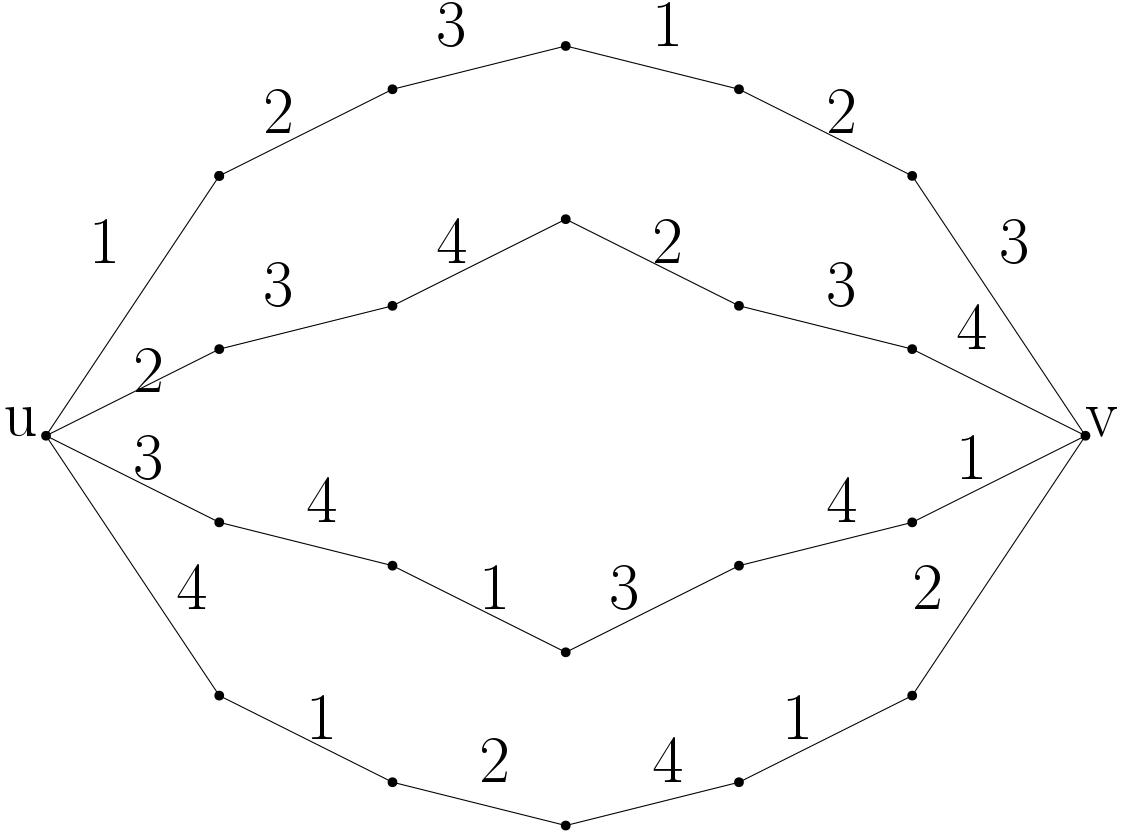
\includegraphics[width=1\linewidth]{figures/d4.png}
\end{center}
\caption{A counterexample to the analogue of Theorem \ref{3-edge-label} for 4-edge-labelings}
\end{figure}
\end{example}
From Condition 1 we know that every 3-KP-labeling of a 3-cycle is constant (monochromatic). The following result analyzes longer cycles.
\begin{lemma}\label{123123}
Let $C$ be a cycle of length at least 4. A 3-edge-coloring of $C$ with colors 1, 2, 3 is a KP-labeling if and only if
\begin{itemize}
\item either it is a 2-edge-coloring of $C$, or
\item possibly after permuting the labels 1, 2, 3, cycle $C$ contains a cyclically ordered sequence
of 6 distinct (not necessarily consecutive) edges labeled 1, 2, 3, 1, 2, 3, respectively. 
\end{itemize}
\end{lemma}

\begin{proof}
Let us start by proving the right direction. Suppose that $C$ is KP-labeled with an edge-coloring using colors 1, 2 and 3 such that all three labels appear on $E(C)$. Fix a cyclic order $\sigma$ of the edges of $C$. Without loss of generality, $C$ has a pair of consecutive edges in $\sigma$, say $e_1$ and $e_2$, that are labeled 1 and 2 respectively. 

By Lemma~\ref{lemma:cyclenotunique} each label must appear at least twice on $C$. Then, the sequence 1,2,3,3 must appear as a such sequence of the labels of edges in order $\sigma$, we stress it here from the lemma that this order is not necessarily consecutive (we could have something like 1,2,3,1,2,1,2,3). Let $P$ be the maximal subpath of $C$ containing $e_1$ and $e_2$ having no edge labeled 3, and let $e$ and $e'$ be the two edges of $E(C)\backslash E(P)$ incident to an edge in $P$. By the maximality of $P$, edges $e$ and $e'$ are labeled 3 and, since each each label appears twice, they must be distinct. 

Let $P'$ be the subpath of $C$ formed by the edges not in $E(P)\cup \{ e,e'\}$. Since $P$ has only labels 1 and 2, in order not to violate Condition 2 both of these labels must appear in $E(C)\backslash E(P)$ and since $e,e' \in E(C)\backslash E(P)$ are labeled 3, it follows that labels 1,2 must appear in $E(P')$. If labels 1 and 2 appear in order $\sigma$ on $P'$ (not necessarily consecutively), we are done. 

Suppose then that all occurrences of 2 appear in $\sigma$ before all occurrences of 1 on $E(P')$. If on $P$ there is an occurrence of label 2 appearing (in $\sigma$) before an occurence of 1, we are done again. By way of contradiction  ,suppose that this is not the case, that is, suppose that all occurces of 1 appear (in $\sigma$) before all occurences of 2 on $P$. \newline
Then $C$ can be divided in two parts in such a way that the occurrences of 1 appear only in one part and the occurences of 2 in the other part, which will violate Condition~2.\newline
Now let us prove the other direction. Since there are no triangles, Condition 1 is satisfied. \newline
If $C$ is 2-edge-labeled, then clearly Condition 2 holds.\newline
Suppose now, without loss of generality, that $C$ contains a cyclically ordered sequence of 6 distinct (not necessarily consecutive) edges labeled 1, 2, 3, 1, 2, 3, respectively. Let $F$ denote a fixed set of 6 edges with the above property. 

Consider now an arbitrary pair $u,v$ of non-adjacent vertices of $C$. Let $P$ and $Q$ be the two $u,v-$subpaths of $C$. At least one of $P$ and $Q$, say $P$, contains at least three consecutive edges from $F$. Hence, any two distinct labels appearing on $Q$ will appear on every induced $u,v$-path. Since this is true for an arbitrary pair $u,v$ of nonadjacent verices, Condition~2 is satisfied.\qedhere


\end{proof}

\section{NP-completeness of testing realizability in $d\geq 3$ dimension}
In this section we will present a result due to Milani\v c, Mur\v si\v c, and Mydlarz in \cite{Milanic}.\newline
We try to understand the question: How difficult is it to determine if a given graph $G$ can be realized in $\mathbb{R}^d$?\newline
We show that for $d=3$, determining whether $Cdim(G)\leq 3$ is NP-complete and for $d\geq 3$ it was shown in \cite{Milanic} that determining whether a given graph $G$ satisfies $Cdim(G) \leq d$ is NP-complete, even for connected bipartite graphs.

\begin{theorem}
Given a graph $G$, determining whether $Cdim(G) \leq 3$ is NP-complete, even for connected bipartite graphs of maximum degree at most 3.
\end{theorem}
\begin{proof}
A polynomially checkable certificate of the fact that $Cdim(G) \leq 3$ is any 3-realization of $G$ of the form $\varphi _G : V \to \{1,2,\ldots, |V(G)|\}^3$, we know that $|\varphi_G(v)|$ is polynomial in $|V(G)|$ for all $v\in V(G)$ as it is cubical. Therefore, the problem is in NP (on any class of input graphs).\newline
In \cite{Ian} it was showed that it is NP-complete to determine the chromatic index of an arbitrary graph. The problem remains NP-complete even for cubic graphs, so to show hardness, we make a reduction from the 3-edge-coloring problem in cubic graphs.\newline
Let $G$ be a cubic graph that is the input for the
3-edge-coloring problem. We may assume that $G$ is connected. Construct a graph $G'$ from $G$ by replacing each edge $xy$ of $G$ with the structure shown in Figure \ref{gadget}, such structure we will call XVWY.

\begin{figure}[h]
\begin{center}
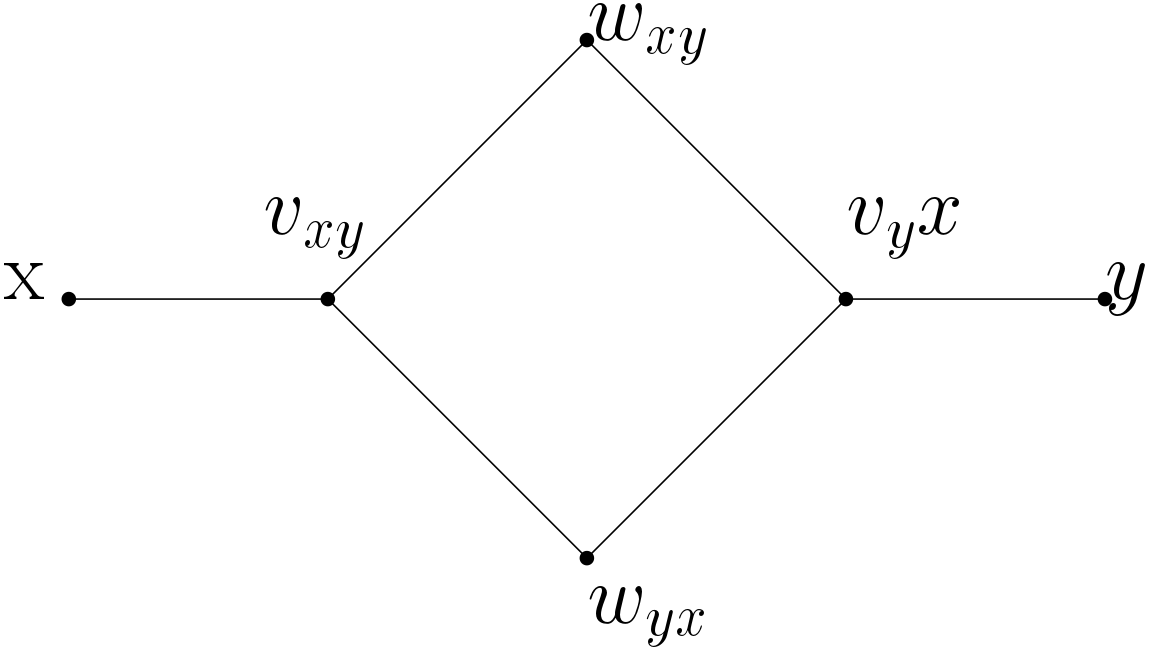
\includegraphics[width=0.6\linewidth]{figures/gadget.png}
\end{center}
\caption{A gadget XVWY replacing each edge $xy$}\label{gadget}
\end{figure}
Formally,
$$V(G')= V(G)\cup
\bigcup_{xy\in E(G)} \{v_{xy}, v_{yx}, w_{xy}, w_{yx}\},$$
$$E(G')=\bigcup_{xy\in E(G)} \{xv_{xy}, v_{xy}w_{xy}, v_{xy}w_{yx}, v_{yx}w_{xy},v_{yx}w_{yx}, yv_{yx}\}.$$
Now let us show that $G'$ is bipartite. Letting $V_1=V(G)\cup
\bigcup_{xy\in E(G)} \{w_{xy},w_{yx}\}$ and $V_2=\bigcup_{xy\in E(G)} \{v_{xy},v_{yx}\}$, we see that $(V_1, V_2)$ is a bipartition of $G'$ since both $V_1$ and $V_2$ are indepedent sets (that is, every possible edge in $G'$ is between $V_1$ and $V_2$). Thus, $G'$ is a bipartite graph with vertices of degrees 2 and 3 only. We will show that $G$ is 3-edge-colorable if and only if $Cdim(G') 
\leq 3$.\newline
Let us show the backward direction. Let $Cdim(G')\leq 3$. By Theorem \ref{thm:mainkp}, $G'$ has a 3-KP-labeling. Then by Lemma \ref{123123} we infer that the cycle $C=v_{xy}-w_{xy}-v_{yx}-w_{yx}-v_{xy}$ in $G'$ must be 2-KP-labled. Since we have 3-KP-labeling, this implies that the edges $xv_{xy}$ and $yv_{yx}$ must have the same label $l_{xy}$, different from labels used in $C$.

 Since $G'$ is triangle-free, any KP-labeling of $G'$ is an edge-coloring (otherwise, Condition 4 would be violated). Therefore, by labeling each edge $xy \in E(G)$ with $l_{xy}$, we get a 3-edge-coloring of $G$.\newline
Now suppose that $G$ has a 3-edge-coloring using colors 1, 2, 3. For each edge $xy$ of $G$ labeled $i \in \{1, 2, 3\}$, let $\{j, k\} = \{1, 2, 3\} \backslash \{i\}$ and label the associated edges of $G'$ as follows: edges $xv_{xy}$ and $yv_{yx}$ with $i$, edges $v_{xy} w_{xy}$ and $v_{yx} w_{yx}$ with $j$, and edges $v_{xy} w_{yx}$ and $v_{yx} w_{xy}$ with $k$.

 We claim that the so obtained labeling of $G'$ is a KP-labeling. Since we have a 3-edge-labeling of $G'$, by Thoerem \ref{3-edge-label}, it suffices to check that Conditions 3 and 4 are satisfied. First we check that no induced $P_3$ is monochromatic. If the edges are stricly from one gadget XVWY then it follows from the labeling that no $P_3$ there is monochromatic. 
 
 If $P_3$ is formed from two gadgets XVWY having a vertex in common, the labels of this $P_3$ are taken from the incident edges in $G$, but the label in $G$ is 3-edge-coloring and it has no monochromatic $P_3$, therefore Condition 4 holds.
In order to verify that Condition 3 holds, note that $G'$ has two types of induced cycles:
\begin{enumerate}
\item[-] 4-cycles. They only appear in the gadget XVWY; they are properly 2-edge-colored and hence KP-labeled by Lemma \ref{123123}.
\item[-] Cycles of length greater than 4. Each such cycle $C$ has length $4p$ for some $p \geq 3$ because the cycle must close in some vertex from set $V(G)$ and by a simple counting argument we get that it must be of length $4p$, and arises from a (not necessarily induced) $p$-cycle $C'$ in $G$. 

We will show that such cycles satisfy the 123123-condition and apply Lemma \ref{123123}. Let $x_1, x_2,\ldots, x_p$ be a cyclic order of vertices in $C'$. Without loss of generality, let 1, 2, 3, 1 be the labels (in this order) on some shortest path from $x_1$ to $x_2$ in $C$. We consider what are possible labels on the edges of any shortest path from $x_2$ to $x_3$ in $C$. 

Since some shortest path from $x_1$ to $x_2$ ends with label 1, no shortest path from $x_2$ to $x_3$ starts with 1, therefore it must start with 2 or 3. If it starts with 2, it must end with labels 1,3,2 or 3,1,2; else if it starts with 3, it must end with labels 1,2,3 or 2,1,3. In every case we can find labels 2,3 in this order and thus, along cycle $C$ we find 6 distinct edges labeled 1, 2, 3, 1, 2, 3 in order. This shows that $C$ satisfies the 123123-condition.
\end{enumerate}
It follows that Condition 3 is satisfied, hence by Theorem \ref{3-edge-label} $G'$ has a 3-KP-labeling. By Theorem \ref{thm:mainkp}, we conclude that $Cdim(G') \leq 3$.  
\end{proof}

\section{Cartesian dimension of grid graphs}
A two-dimensional grid graph is the Cartesian product two path graphs. The results below will demonstrate that when finding the exact Cartesian dimension of these graphs and for paths of length at least 3, the Cartesian dimension is the same for any pair of path graphs, namely 4. To prove these results, we will use the Theorem \ref{thm:mainkp} which can be understood as follows for a connected graph $G$ and positive integer $d$, $Cdim(G) \leq d$ if and only if $G$ has a $d$-KP-labeling.\newline
\begin{theorem}
\[
	\Cdim(P_i \square P_j ) =
		\left\{
			\begin{array}{ll}
				0, & \text{if $(i,j)=(1,1)$;} \\
				1, & \text{if $(i,j)\in \{(1,2),(2,1)\}$;} \\
				2, & \text{if $(i,j)\in \{(2,2)\} \cup \{(1,k)|k\geq 3\} \cup \{(k,1)|k\geq 3\}$;} \\
				3, & \text{if $(i,j)\in \{(2,k)|k\geq 3\} \cup \{(k,2)|k\geq 3\}$;} \\
				4, & \text{if $(i,j)\in \{(k,l)|k,l\geq 3\}$;}
			\end{array}
		\right.
\]
\end{theorem}
\begin{proof}

 Without loss of generality, we may assume that $i\leq j$.\newline
 If $i=1$, then $P_1\square P_j\cong P_j$; if $j=1$ then there is no edges, therefore $Cdim(P_i\square P_j)=0$; if $j=2$, then there is only one edge, therefore $Cdim(P_i\square P_j)=1$; and if $j\geq 2$, then alternate by following the path horizontal and vertical in $\mathbb{R}^2$, therefore $Cdim(P_i\square P_j)=2$.\newline 
If $i=2$ and $j=2$, then $Cdim(P_i\square P_j)=2$.
\newline
If $j\geq 3$, from Theorem \ref{d-realizable-free}, we have that $Cdim(P_2\square P_j)\geq 3$, since $P_2 \square P_j$ has $K_{1,3}$ as induced subgraph.\newline
Next, we find a $KP$-labeling of the graph with 3 labels.
\begin{figure}[h]
\begin{center}
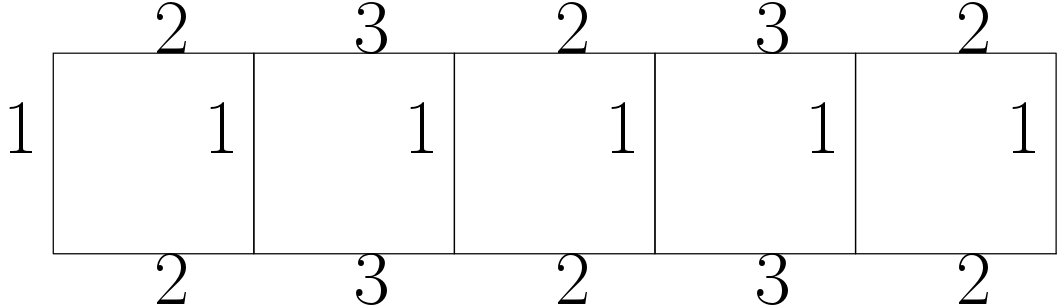
\includegraphics[width=1\linewidth]{figures/p_2sqp_j.png}
\end{center}
\caption{KP-labeling of $P_2\square P_6$}\label{fig:P_2sqP_6}
\end{figure}\newline
We label the copies of the first factor ($P_2$) with label 1 and both copies of $P_j$ the same by alternating between 2 and 3.
An example of how we label $P_2\square P_6$ is shown in Figure \ref{fig:P_2sqP_6}.\newline
For any two nonadjacent vertices, $u$ and $v$, if they belong to a $C_4$, we take label 1 and the other label from set $\{2,3\}$ to satisfy Condition 2. 

If they do not belong to some $C_4$, then we take labels 2 and 3. Note that $u$ and $v$ are in different components when taking the partition of graph with respect to labels 2 or 3, meaning that every induced $u,v$-path has an edge labeled $i$, for $i$ in $\{2,3\}$.\newline
Therefore, this labeling is a KP-labeling and from Theorem \ref{thm:mainkp}, we have that $Cdim(P_2\square P_j)\leq 3$.\newline
Combining both inequalities, we have that $Cdim(P_2\square P_j)=3$ if $j\geq 3$.

Finally, we look at the case $i\geq 3$.
\newline
If $i\geq 3$, from Theorem \ref{d-realizable-free}, we have that $Cdim(P_i\square P_j)\geq 4$, since $P_i \square P_j$ has $K_{1,4}$ as induced subgraph.\newline
Next, we find a KP-labeling of the graph with 4 labels.
\begin{figure}[h]
\begin{center}
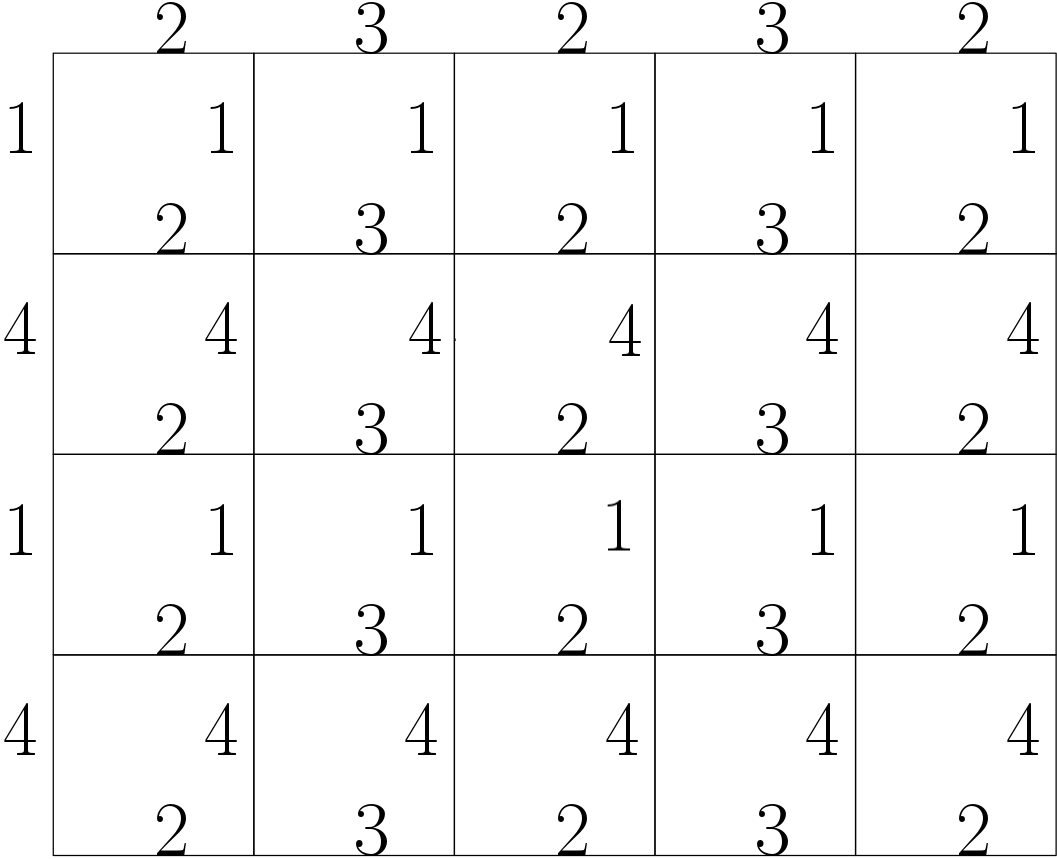
\includegraphics[width=1\linewidth]{figures/p_isqp_j.png}
\end{center}
\caption{KP-labeling of $P_5\square P_6$}
\end{figure}\newline
We label the copies of $P_i$ identically by alternating between 1 and 4; and the copies of $P_j$ identically by alternating between 2 and 3.\newline
For any two nonadjacent vertices, $u$ and $v$, when they belong to a $C_4$, we take the two labels in this cycle. However, if any two nonadjacent vertices, $u$ with coordinates $(a,x)$ and $v$ with coordinates $(b,y)$, do not belong to a $C_4$, then either $d_{P_i}(a,b) \geq 2$ or $d_{P_j}(x,y) \ge 2$. 

If $d_{P_i}(a,b) \geq 2$, we take labels 2 and 3; otherwise, we take labels 1 and 4. Similarly to the previous proposition, vertices $u$ and $v$ would belong to different components when removing either of the choosen labels. 
 \newline
Therefore, this label is a KP-labeling and from Theorem \ref{thm:mainkp}, we have that $Cdim(P_i\square P_j)\leq 4$.\newline
Combining both inequalities, we have that $Cdim(P_i\square P_j)=4$, if $i\geq 3$.
\end{proof}

\chapter{Hamming dimesion}\label{hdim-chapter}
Graph products offer a variety of possibilities to introduce the concept of a graph dimension. A classical result of Graham and Winkler \cite{Graham} shows that any graph can be canonically isometrically embedded into the Cartesian product of graphs. Knowing that, this embedding is unique among all irredundant isometric embeddings with respect to the largest possible number of factors. The latter number is is defined to be the \textit{isometric dimension} of a graph. 
\newline The strong product $G\boxtimes H$ of graphs $G$ and $H$ is a graph such that the vertex set of $G\boxtimes H$ is the Cartesian product $V(G) \times V(H)$; distinct vertices $(u,u')$ and $(v,v)$ are adjacent in $G\boxtimes  H$ if and only if $u = v$ and $u'$ is adjacent to $v'$, or $u' = v'$ and $u$ is adjacent to $v$, or $u$ is adjacent to $v$ and $u'$ is adjacent to $v'$.

 Back in 1938 Sch\" onberg \cite{Schonber} proved that every connected graph admits an isometric embedding into the strong product of paths. It is hence natural to define the \textit{strong isometric dimension}, $idim(G)$, of a graph $G$ as the least number $k$ such that $G$ embeds isometrically into the strong product of $k$ paths.\newline
Eppstein considered the following representation problem in \cite{David}: to which unweighted undirected graphs one can assigned integer coordinates in some $d$-dimensional space $\mathbb{Z}^d$ such that the distance between two vertices in the graph is equal to the $L_1$-distance (taxicab) between their coordinates? Call the minimum possible dimension $d$ of such an embedding (if one exists) the \textit{lattice dimension} of the graph.\newline
The strong isometric dimension is universal in the sense that as soon as a graph is not the path graph, then its dimension is finite and bigger than 1. A similar conclusion can be stated for the so called direct dimension of a graph defined in \cite{Eaton}.

 On the other hand, for one of the most important graph products, the Cartesian product, no such universal dimension is known. While the isometric dimension is useful as soon as the dimension of a graph is more than 1, it was proved in \cite{Poljak} that almost all graphs have isometric dimension 1. In other words, for almost all graphs $G$ the isometric dimension yields no new insight about $G$. Also, only the so called partial cubes, a special (although important) subclass of bipartite graphs, have finite lattice dimension.\newline
\newline
To significantly increase the number of graphs with a non-trivial dimension, Klav\v zar, Peterin, and Zemlji\v c, defined in \cite{Sandi} the \textit{Hamming dimension} $Hdim(G )$ of a graph $G$ as the largest dimension of a Hamming graph into which $G$ embeds as an irredundant induced subgraph. If $G$ is not an induced subgraph of any Hamming graph, we set $Hdim ( G ) = \infty$.\newline In Figure \ref{fig:c6hdim} we shown the 6-cycle, as an induced subgraph of two different Hamming graphs, $K_3\square K_3$ and $K_2\square K_2\square K_2$.
\begin{figure}[h]
\begin{center}
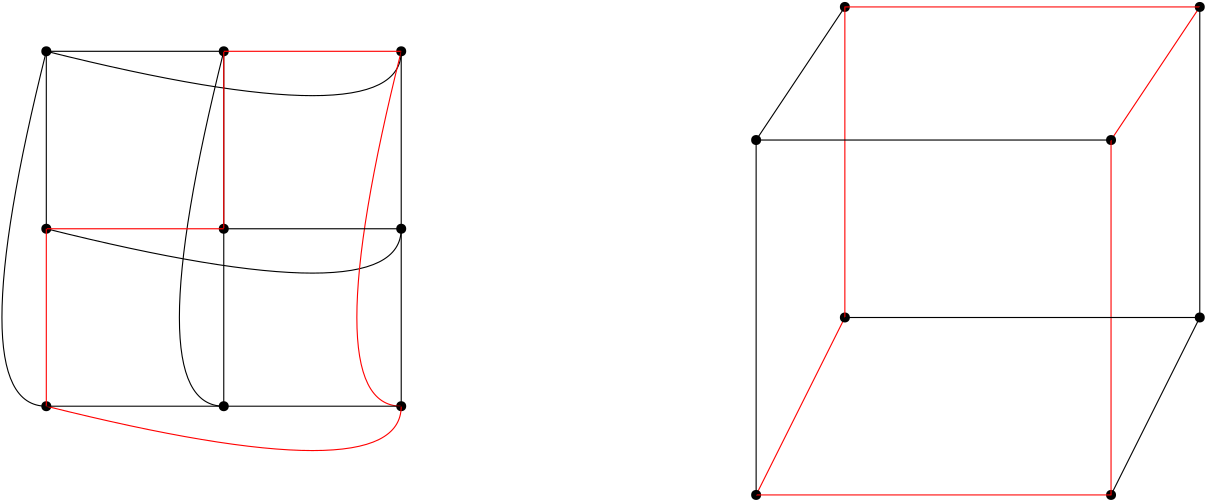
\includegraphics[width=1\linewidth]{figures/c_6hdim.png}
\end{center}
\caption{$C_6$ induced in $K_3\square K_3$ and $K_2\square K_2\square K_2$}\label{fig:c6hdim}
\end{figure}
Clearly, $Hdim ( G ) = 1$ if and only if $G$ is a complete graph. From Theorem~\ref{thm:mainkp}, we infer that $Hdim ( G ) <\infty$ if and only if $G$ has a "KP-labeling".
\section{Hamming dimension of Sierpi\' nski graphs}
The general problem of determining the Hamming dimension of a graph seems very challenging. Here we will study this concept on Sierpi\' nski graphs. Roughly speaking, in \cite{Sandi}, they proved that all Sierpi\'nski graphs (except in the trivial cases) have Hamming dimension bigger than 1 and finite. 

On the other hand, all but base 3 Sierpi\'nski graphs have isometric dimension 1. \newline
Graphs whose drawings can be viewed as approximations to the famous Sierpi\'nski triangle have been studied intensely in the past 25 years. The interest for these graphs comes from many different sources such as games like the Chinese rings or the Tower of Hanoi, topology, physics, the study of interconnection networks, and elsewhere.\newline
Sierpi\'nski graphs $S^{k}_n$ were studied for the first time by Klav\v zar and Milutinovi\' c in \cite{Sandi2}. In computer science, a very similar class of graphs (known as WK-recursive networks) was introduced earlier by Vecchia and Sanges in \cite{Vecchia}. 

The study in \cite{Sandi2} was motivated in part by the fact that for $k=3$ these graphs are isomorphic to the Tower of Hanoi graphs and in part by topological studies.\newline
A 1-perfect code in a graph $G$ is a vertex subset of $G$ with the property that the closed neighborhoods of its elements form a partition of $V(G)$. The graphs $S^k_n$ were investigated from numerous points of view, we recall some of them. These graphs contain unique 1-perfect codes, proven by Klav\v zar, Milutinovi\' c, and Petr in \cite{Ciril}. 

Metric properties of Sierpi\'nski graphs were investigated in \cite{Andreas}. To
determine the chromatic number of these graphs is easy, while in \cite{Andreas2} it is proved that they are in
edge- and total coloring class 1, except those isomorphic to a complete graph of odd or even order, respectively.\newline
The Sierpi\'nski graph $S^k_n$, where $k,n\geq 1$, is defined on the vertex set $\{ 1,\ldots,k \}^n$ , two different vertices $u = (u_1 ,\ldots, u_n )$ and $v = (v_1 ,\ldots , v_n)$ being adjacent if and only if there exists an $h \in \{ 1 , \ldots, n \}$ such that
\begin{enumerate}[label=(\roman*)]
\item $u_t = v_t$ , for $t = 1 ,\ldots , h-1$;
\item $u_h \neq v_h$ ; and
\item $u_t = v_h$ and $v_t = u_h$ for $t = h+1 ,\ldots, n$.
\end{enumerate}
An example of Sierpi\'nski Graph is shown in Figure \ref{fig:spierpinski}.
\begin{figure}[h]
\begin{center}
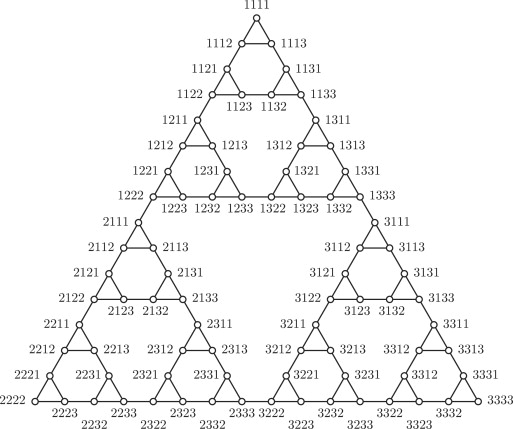
\includegraphics[width=1\linewidth]{figures/sierpinski.png}
\end{center}
\caption{The Sierpi\'nski graph $S^3_3$}\label{fig:spierpinski}
\end{figure}
Below we will state without proof some results from \cite{Sandi}.

\begin{theorem}
For any $n\geq 2$
$$Hdim( S^3_n)\geq \frac{7}{4}\cdot 3^{n-3}+3\cdot 2^{n-4}+\frac{3}{2}\cdot n-\frac{9}{4}.$$
\end{theorem}

\begin{proposition}
\begin{enumerate}[label=(\roman*)]
\item $Hdim(S_3^2)=3,Hdim(S_3^3)=6$.
\item For any $k\geq 4$, $Hdim(S_k^2)=2$. 
\end{enumerate}
\end{proposition}

\begin{theorem}
\begin{enumerate}[label=(\roman*)]
\item $Hdim(S_3^n)\leq 5\cdot 3^{n-3}+1$ for all $n\geq 3$.
\item $Hdim(S_k^n)\leq \frac{2}{k-1}k^{n-2}+\frac{2k-4}{k-1}$ for all $k\geq 4 \text{ and } n\geq 2$. 
\end{enumerate}
\end{theorem}

\begin{corollary}
For any $k\geq 4$, $Hdim(S_k^3)=4$.
\end{corollary}

\chapter{Conclusion}
This project paper is focused on carefully examining the representations of graphs as induced subgraphs of Hamming graphs. We have seen that a graph $G$ is an induced subgraph of a Hamming graph if and only if there exists a labeling of $E(G)$ fulfilling the two conditions:\begin{enumerate}
\item edges of a triangle receive the same label,
\item for any vertices $u$ and $v$ at distance at least two, there exist two labels which both appear on any induced $u; v$-path. 
\end{enumerate}
We have noticed that for Cartesian dimension, the two-dimensional case corresponds to the class of line graphs of bipartite graphs and is well-understood, while for all $d\geq 3$ the problem of determining whether a given graph $G$ is $d$-realizable is NP-complete.\newline
Shortly, we also defined the Hamming dimension and stated without proofs some statements.\newline
It would be interesting to perform a further study and comparison of the Cartesian and the Hamming dimension of graphs for graphs of particular classes, such as planar graphs or graphs of small maximum degree, as well as for more structed graph families such as generalized Petersen graphs, Johnson graphs, etc. 

 \begin{thebibliography}{99}
\thispagestyle{fancy}

\bibitem{Bermond}
  \articleInJournalManyAuthors
    {Jean-Claude Bermond, Marie-Claude Heydemann}{Dominique Sotteau}
    {Line graphs of hypergraphs}
   {Discrete Math}{18}
   {1977}{235--241} 


\bibitem{Cook}
  \articleInJournalOneAuthor
    {Curtis R. Cook}
    {Representations of graphs by $n$-tuples}
   {In Proceedings of the Fifth Southeastern Conference on Combinatorics, Graph Theory, and Computing}{10}
   {1974}{303--316}

\bibitem{Eaton}
  \articleInJournalManyAuthors
    {Nancy Eaton}{Vojt\v ech R\" odl}
    {Graphs of small dimensions}
   {Combinatorica}{16}
   {1996}{59--85}

\bibitem{Egawa}
  \articleInJournalOneAuthor
    {Yoshimi Egawa}
    {Characterization of the Cartesian product of complete graphs by convex subgraphs}
   {Discrete Mathematics}{58}
   {1986}{307--309}     

\bibitem{David}
\articleInJournalOneAuthor
    {David Eppstein}
    {The lattice dimension of a graph}
   {European Journal of Combinatorics}{26}
   {2005}{585--592} 

\bibitem{Feder}
\articleInJournalOneAuthor
    {T. Feder}
    {Product graph representations}
   {Journal Graph Theory}{16}
   {1992}{467--488}

\bibitem{Graham}
  \articleInJournalManyAuthors
    {R.L. Graham}{P.M. Winkler}
    {On isometric embeddings of graphs}
   {American Mathematical Society}{288}
   {1985}{527--536}

\bibitem{Gurvich}
  \articleInJournalManyAuthors
    {Vladimir A. Gurvich}{Mikhail A. Temkin}
    {Cellular perfect graphs}
   {Dokl. Akad. Nauk}{362}
   {1992}{527--536}

\bibitem{Andreas2}
  \articleInJournalManyAuthors
    {Andreas M. Hinz}{Daniele Parisse}
    {Coloring Hanoi and Sierpiński graphs}
   {Discrete Mathematics}{312}
   {2012}{1521--1535}  

\bibitem{Andreas}
  \articleInJournalManyAuthors
    {Andreas M. Hinz}{Daniele Parisse}
    {The Average Eccentricity of Sierpi\' nski Graphs}
   {Graphs and Combinatorics}{28}
   {2012}{671--686}

\bibitem{Ian}
\articleInJournalOneAuthor
    {Ian Holyer}
    {The NP-completeness of edge-coloring}
   {SIAM J. Comput.}{10}
   {1981}{718--720}  

\bibitem{Imrich}
  \articleInJournalManyAuthors
    {Wilfried Imrich} {Sandi Klav\v zar}
    {Recognizing Hamming graphs in linear time and space}
   {Information Processing Letters}{63}
   {1997}{91--95}

\bibitem{Iztok}
  \articleInJournalManyAuthors
    {Sandi Klav\v zar}{Iztok Peterin}
    {Characterizing subgraphs of Hamming graphs}
   {Journal of Graph Theory}{49}
   {2005}{302--312} 

\bibitem{Sandi}
  \articleInJournalManyAuthors
    {Sandi Klav\v zar, Iztok Peterin}{Sara Sabrina Zemlji\v c}
    {Hamming dimension of a graph-The case of Sierpi\'nski graphs}
   {European Journal of Combinatorics}{34}
   {2013}{460--473}

\bibitem{Sandi2}
  \articleInJournalManyAuthors
    {Sandi Klav\v zar}{Uro\v s Milutinovi\' c}
    {Graphs $S(n, k)$ and a Variant of the Tower of Hanoi Problem}
   {Czechoslovak Mathematical Journal}{47}
   {1997}{95--104}

\bibitem{Ciril}
  \articleInJournalManyAuthors
    {Sandi Klav\v zar, Uro\v s Milutinovi\' c}{Ciril Petr}
    {1-perfect codes in Sierpi\' nski graphs}
   {Bulletin of the Australian Mathematical Society}{66}
   {2002}{}


\bibitem{Milanic}
  \articleInJournalManyAuthors
    {M. Milani\v c, P. Muršič}{M. Mydlarz}
    {Induced Embeddings into Hamming Graphs}
   {42nd International Symposium on Mathematical Foundations of Computer Science}{83}
   {2017}{1--15}   

\bibitem{Mollard}
  \articleInJournalOneAuthor
    {Michel Mollard}
    {Two characterizations of generalized hypercube}
   {Discrete Mathematics}{93}
   {1991}{63--74}

\bibitem{Mulder}
  \articleInJournalOneAuthor
    {Henry Martyn Mulder}
    {Interval-regular graphs}
   {Discrete Mathematics}{41}
   {1982}{253--269}  

\bibitem{Peterson}
\articleInJournalOneAuthor
    {Dale Peterson}
    {Gridline graphs: a review in two dimensions and an extension to higher dimensions}
   {Discrete Appl. Math.}{126}
   {2003}{223--239}


\bibitem{Poljak}
  \articleInJournalManyAuthors
    {S. Poljak}{A. Pultr}
    {Representing graphs by means of strong and weak products}
   {Comment. Math. Univ. Carolin.}{22}
   {1981}{449--466} 


\bibitem{Zito}
  \articleInJournalManyAuthors
    {Pavan Sangha}{Michele Zito}
    {Finding Large Independent Sets in Line of Sight Networks}
   {Algorithms and Discrete Applied Mathematics}{10156}
   {2017}{332--343}    

\bibitem{Schonber}
\articleInJournalOneAuthor
    {I.J. Schonber}
    {Metric spaces and positive definite functions}
   {Trans. Amer.Math. Soc.}{44}
   {1938}{522--536}


\bibitem{Staton}
  \articleInJournalManyAuthors
    {William Staton}{G. Clifton Wingard}
    {On line graphs of bipartite graphs}
   {Util. Math.}{53}
   {1998}{183--187}      
   
\bibitem{Vecchia}
  \articleInJournalManyAuthors
    {G.Della Vecchia}{C. Sanges}
    {A recursively scalable network VLSI implementation}
   {Future Generation Computer Systems}{4}
   {1988}{235--243}    
        
% There has to be an empty line here so that the page numbers of citations are properly displayed.
\end{thebibliography}
\newpage

%%%%%%%%%%%%%%%%%%%%%%%%%%%%%%%%%%%% Appendices %%%%%%%%%%%%%%%%%%%%%%%%%%%%%%%%%%%%%

\pagestyle{fancyplain}
\vspace*{\fill}
     \begin{center}
          \bf{\Huge{Appendices}}
     \end{center}
\vspace*{\fill}
\thispagestyle{fancy}

\appendix
\thispagestyle{empty}
\pagenumbering{gobble}

\addtocontents{toc}{\setcounter{tocdepth}{-1}}
\appendices{A Title of First Appendix}
\chapter{Title of First Appendix}
\thispagestyle{empty}

\begin{lemma}\label{diamondmost}
If $C$ is a maximal clique in a diamond-free graph $G$ and $v\in V(G)\backslash C$, then $v$ has at most one neighbor in $C$.
\end{lemma}
\begin{proof}
Suppose for a contradiction that $v$ has two neighbors in $C$, say $x$ and $y$. Since $C$ is maximal clique, there exist a vertex in $C$, say $z$, such that is not adjacent to $v$ (otherwise $C\cup \{v\}$ would be a clique properly containg $C$, contradicting the maximality of $C$). But now, vertices $v,x,y,z$ induce a diamond in $G$, a contradiction. 
\end{proof}
\begin{corollary}\label{maxcliquedia}
If $C$ and $C'$ are maximal cliques in a diamong-free graph $G$ such that $C\neq C'$ and $C\cap C'\neq \emptyset$, then $|C\cap C'|= 1$ and there are no edges between vertices of $C\backslash C'$ and vertices of $C'\backslash C$.
\end{corollary}
\begin{proof}
If $|C\cap C'|\geq 2$ then any vertex in $C\backslash C'$ would have more than 2 neighbors in $C'$, contradicting Lemma~\ref{diamondmost}. Thus, $|C\cap C'|=1$. Let $\{v\}= C\cap C'$. If a vertex $x\in C\backslash C'$ is adjacent to a vertex $y\in C'\backslash C$, then $x$ is a vertex not in $C'$ adjacent to at least two vertices in $C'$ (namely, $v$ and $y$), again contradicting Lemma~\ref{diamondmost}
\end{proof}
% Be careful:
% the command
% \thispagestyle{empty}
% has to be present on every page of each appendix (so that the document header is not displayed)

\appendices{B Title of Second Appendix}
\chapter{Title of Second Appendix}
\thispagestyle{empty}

\begin{corollary}
If $G$ is a \{diamond, claw\}-free graph, then every vertex $v\in V(G)$ is contained in at most two maximal cliques.
\end{corollary}

\begin{proof}
Suppose $v\in V(G)$ is contained in at three distinct maximal cliques of $G$, say $C_1,C_2,C_3$. Let $v_i\in C_i\{v\}$ for $i\in \{1,2,3\}$. Then $v,v_1,v_2,v_3$ induce a claw by Corollary~ref{maxcliquedia}, a contradiction.
\end{proof}

% Be careful:
% the command
% \thispagestyle{empty}
% has to be present on every page of each appendix (so that the document header is not displayed)

\addtocontents{toc}{\setcounter{tocdepth}{2}}
\end{document}
